\documentclass[11pt]{article}


% Codificación de caracteres e idioma
\usepackage[utf8]{inputenc}
\usepackage[spanish]{babel}

% Tamaño de página y márgenes
\usepackage[letterpaper, margin=2.5cm]{geometry}

% Orientación horizontal de página
\usepackage{lscape, lscape}

% Comillas, columnas, gráficos, símbolos matemáticos e ingreso de código de programación
\usepackage{csquotes, multicol, graphicx, amssymb, amsmath, listings, xcolor}

% Para tablas grandes y líneas estéticas de tablas
\usepackage{xltabular, booktabs}

% Para hacer mosaico de figuras
\usepackage{subcaption}

% Interlineado 1.5
\usepackage{setspace}
\onehalfspacing

% Uso de punto decimal, en lugar de coma
\decimalpoint

% Separación de columnas y sangría
\setlength{\columnsep}{2cm} 
\setlength{\parindent}{0cm}

% Páginado
\pagestyle{plain}

% Evitar separación de palabras
\hyphenpenalty=10000
\exhyphenpenalty=10000
\sloppy


\begin{document}

\begin{titlepage}
	\centering
	{\scshape\LARGE Universidad Aztlán \par}
	\vspace{1cm}
	{\scshape\Large Campus Playa del Carmen \par}
	\vspace{1.75cm}
	{\scshape\Huge Sistema de Gestión de una Tienda \par}
    \vfill
    {\itshape\Large Proyecto Final \par}
	\vspace{2cm}
    {\itshape\Large Presentado por: \par}
	{\Large José Rosendo Camal Teh \par}
	\vfill
	{\Large Ingeniería en Sistemas Computacionales \par}
	{\Large Cuarto Cuatrimestre \par}
	{\Large Fundamentos de Bases de Datos \par}
	\vfill
	{\Large Profe. Emmanuel Andrés Martínez López \par}
	\vfill
	{\Large 23 de octubre de 2026 \par}
	\vfill
	{\Large Playa del Carmen, Quintana Roo \par}
\end{titlepage}
\newpage


\tableofcontents
\newpage 

\section*{\centering Diagrama Entidad-Relación}
\addcontentsline{toc}{section}{Diagrama Entidad-Relación}
\begin{figure}[!htb]
	\centering
	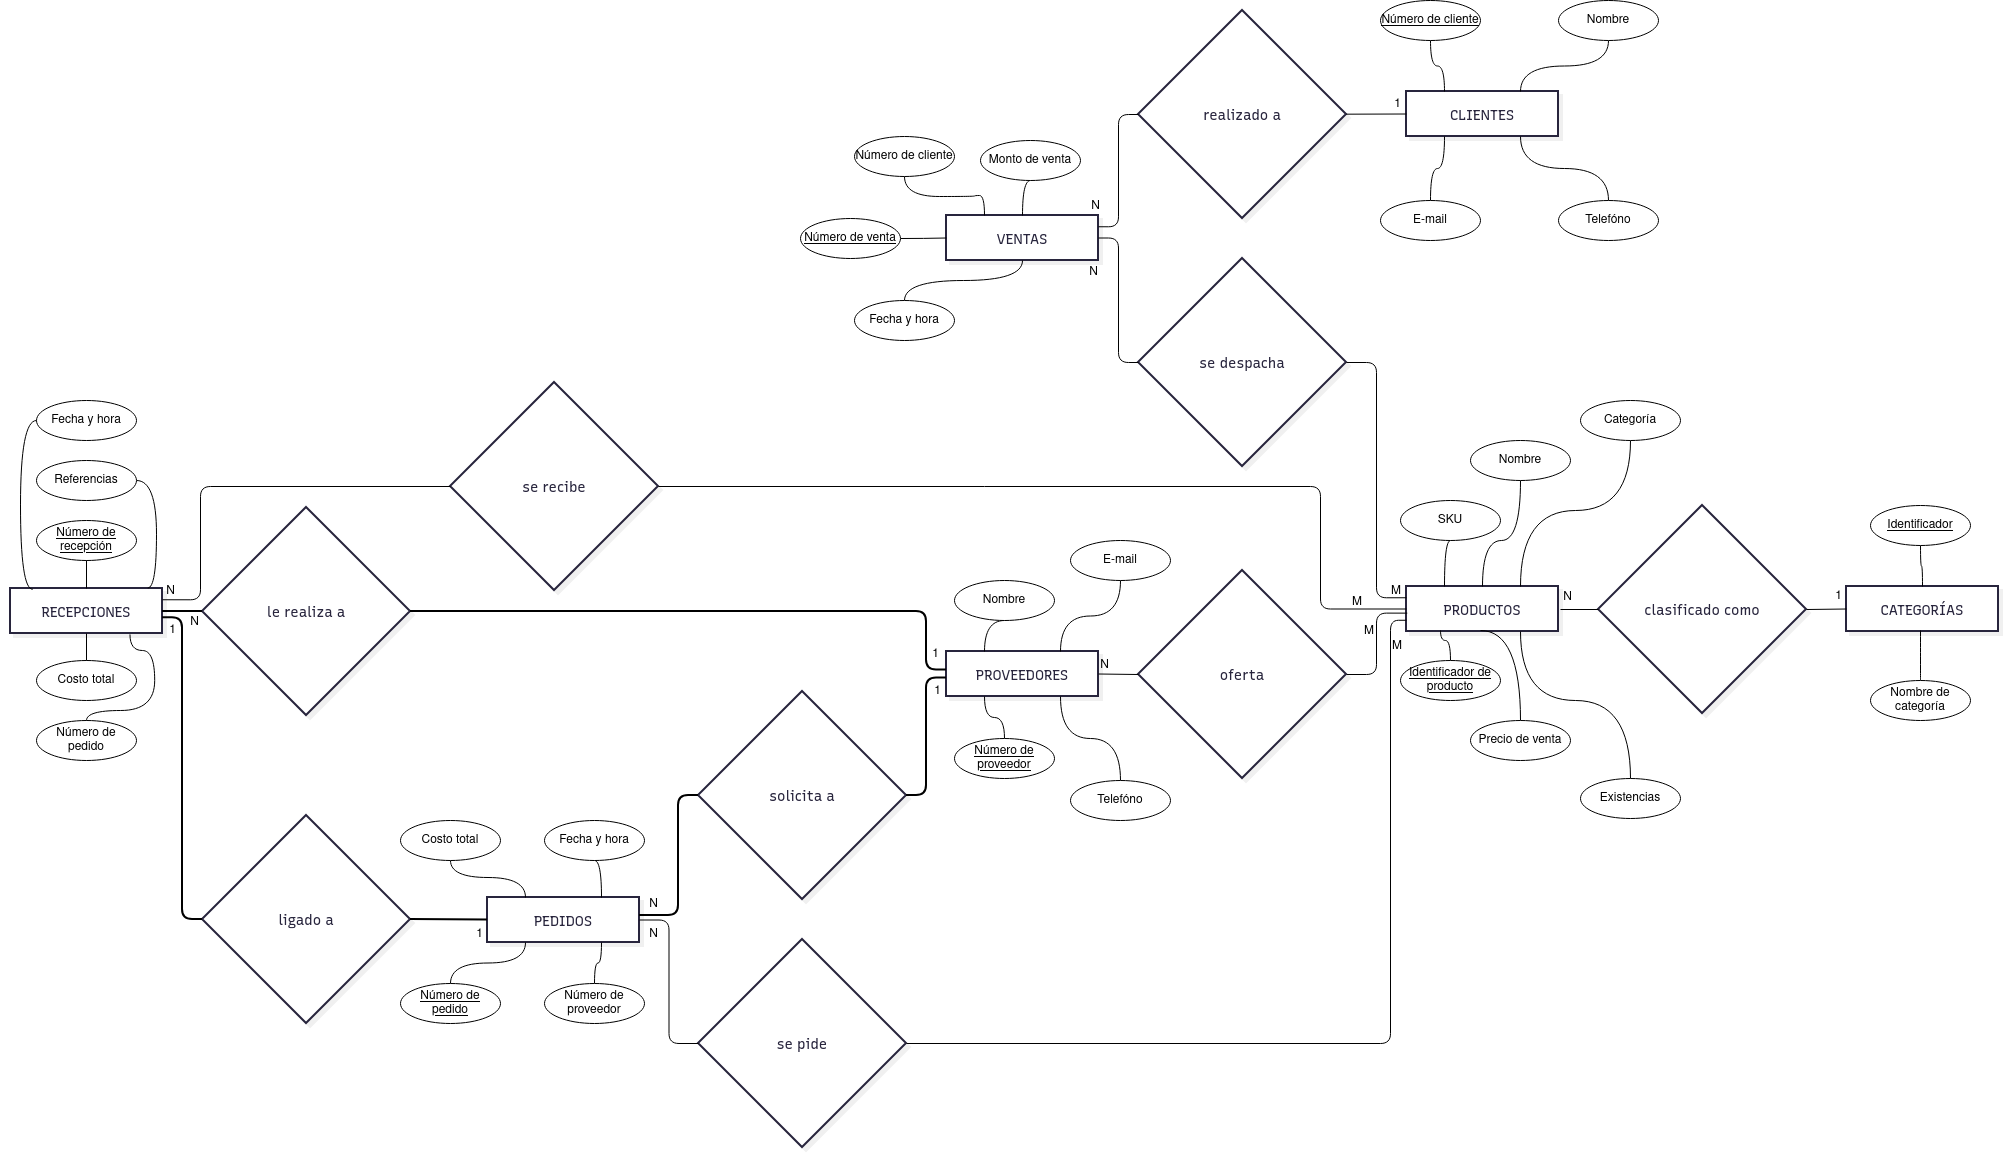
\includegraphics[
        width=0.9\textheight,
        height=0.8\textwidth,
        angle=90
        ]{../img/erDiagram.drawio.png}
	\caption{\textit{Diagrama ER}}
	\label{fig:relationalModel}
\end{figure}
\vfill
\newpage

\section*{\centering Modelo Relacional}
\addcontentsline{toc}{section}{Modelo Relacional}
\vfill
\begin{figure}[!htb]
	\centering
	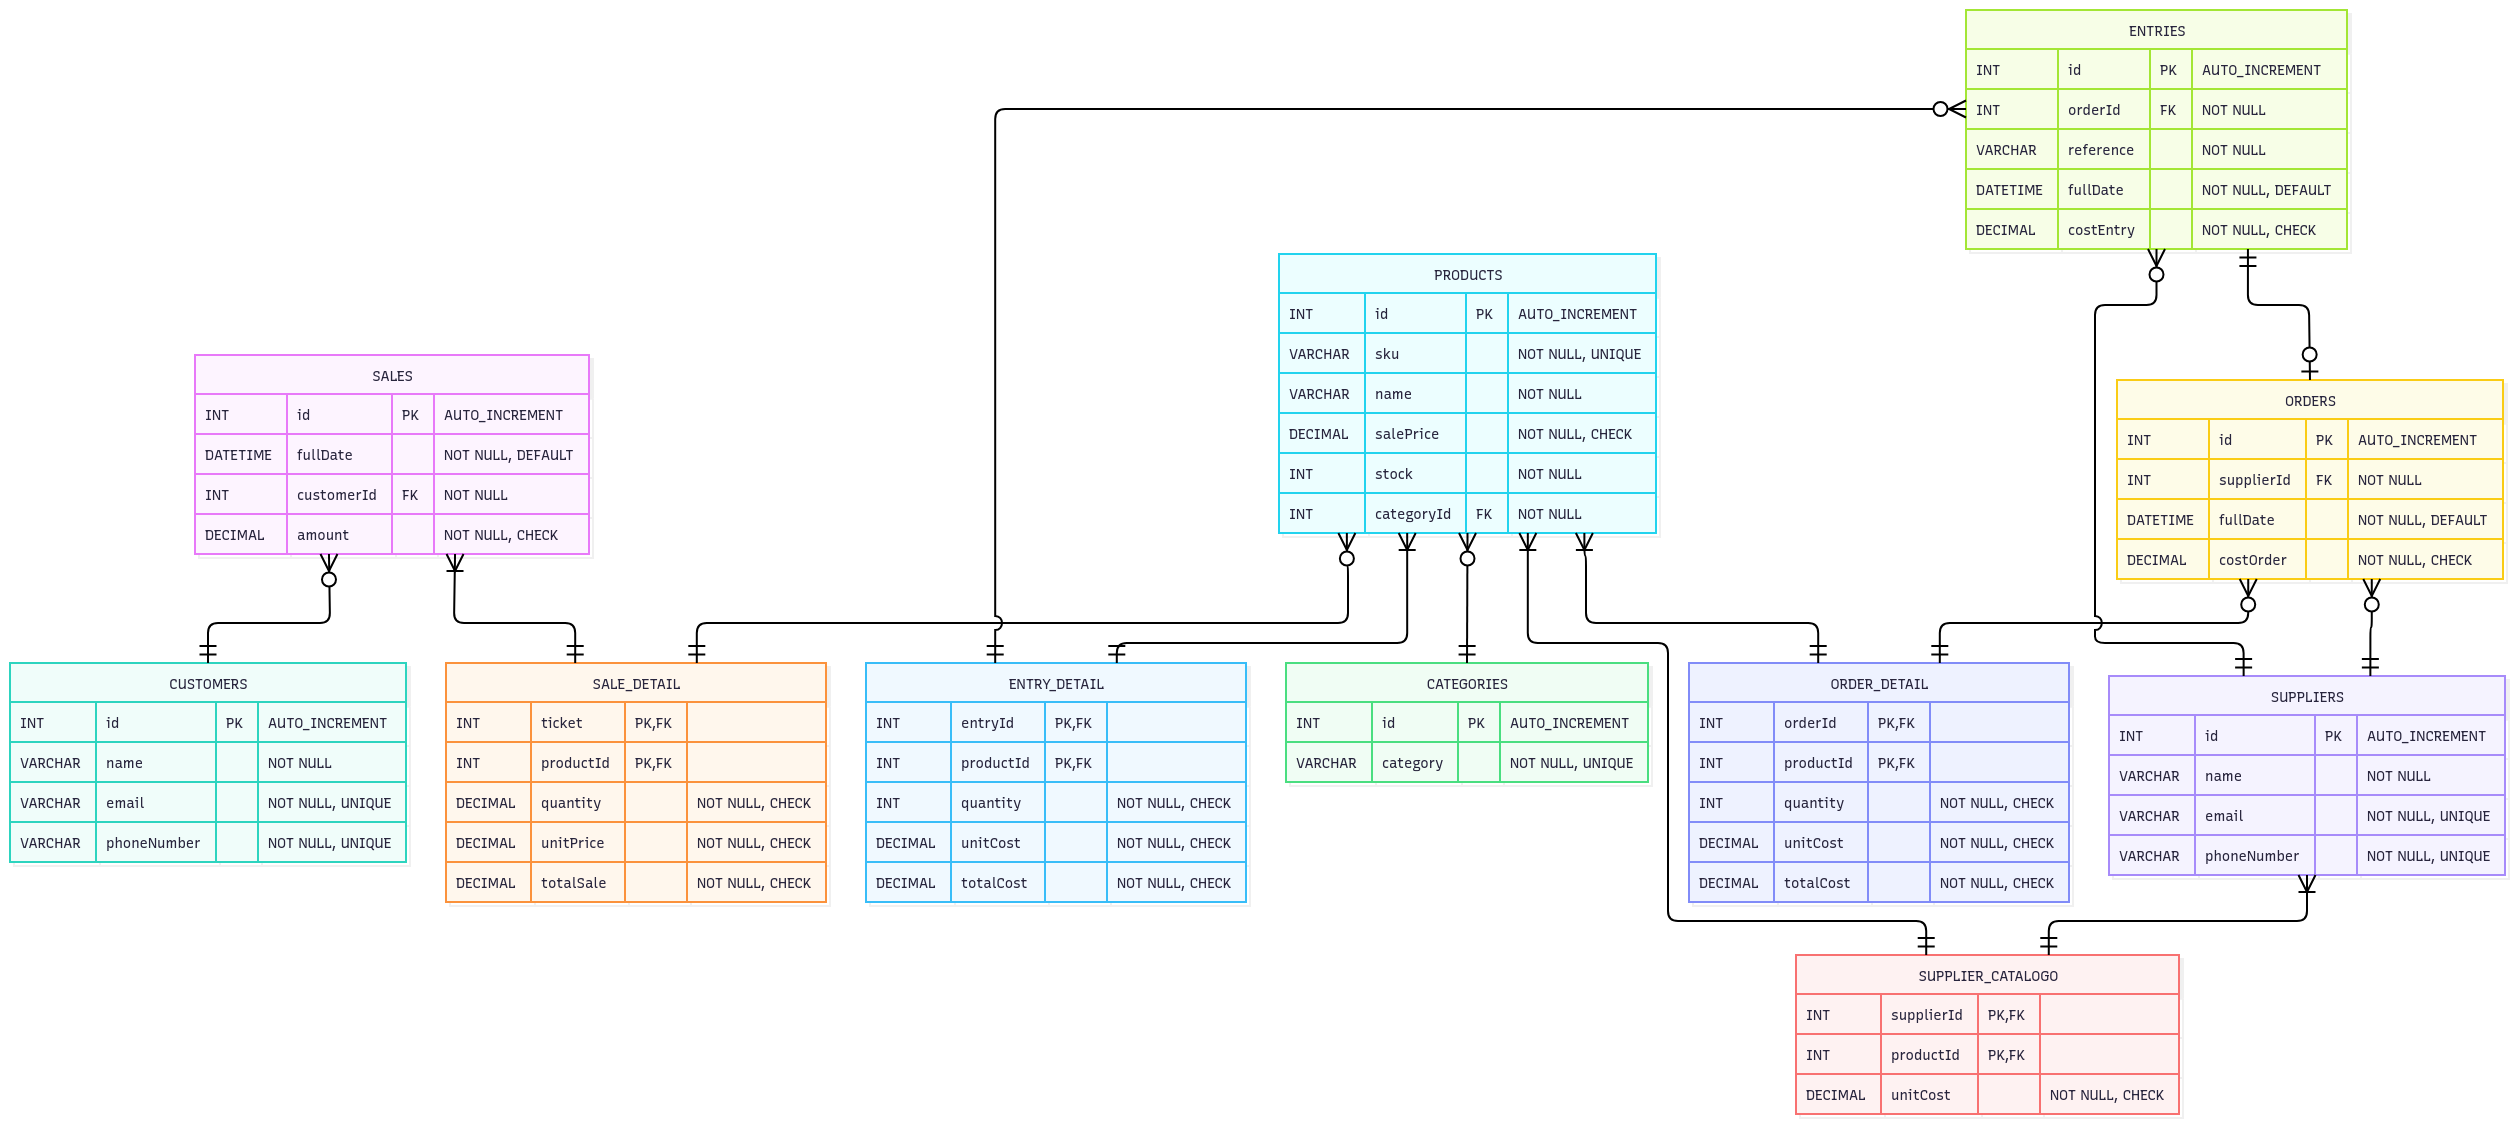
\includegraphics[
        width=0.9\textheight,
        height=0.55\textwidth,
        angle=90
        ]{../img/relationalModel.drawio.png}
	\caption{\textit{Modelo relacional}}
	\label{fig:relationalModel}
\end{figure}
\vfill
\newpage

\section*{\centering Diccionarios de datos}
\addcontentsline{toc}{section}{Diccionarios de datos}
\vspace{0.5cm}
\begin{table}[h!]
\centering
\caption{\textit{Diccionario de datos por entidad}}
\label{tab:diccionario-entidad}
\begin{tabular}{
    | p{3.3cm}
    | p{5.2cm}
    | p{2.8cm}
    | p{2.8cm} |
}
	\toprule
	\textbf{Tabla} & \textbf{Descripción} & \textbf{\texttt{PK}} & \textbf{\texttt{FK}} \\
    \midrule
    \texttt{PRODUCTS}            & Los artículos que vende una tienda, que adquiere el cliente y fabrica o distribuye un proveedor.      & \texttt{id}                               & \texttt{categoryId} \\
    \midrule
    \texttt{SUPPLIERS}           & Los agentes que entregan la mercancía a la tienda para que este lo distribuya y venda.                & \texttt{id}                               & \\
    \midrule
    \texttt{ENTRIES}             & El proceso de una tienda de recibir la mercancía al proveedor.                                        & \texttt{id}                               & \texttt{orderId} \\
    \midrule
    \texttt{ORDERS}              & El proceso de una tienda de solicitar resurtido de mercancía al proveedor.                            & \texttt{id}                               & \texttt{supplierId} \\
    \midrule
    \texttt{SALES}               & Las transacciones entre clientes y la tienda, donde el primero adquiere un artículo usando su dinero. & \texttt{id}                               & \texttt{customerId} \\
    \midrule
    \texttt{CUSTOMERS}           & Los agentes que adquiere los productos ofertados por la tienda.                                       & \texttt{id}                               & \\
    \midrule
    \texttt{CATEGORIES}          & La clasificación de la mercancía según su utilidad, caducidad u otros criterios.                      & \texttt{id}                               & \\
    \midrule
    \texttt{SUPPLIER\_CATALOGO}  & Los productos ofertados por los proveedores.                                                          & \texttt{supplierId}, \texttt{productId}   & \texttt{supplierId}, \texttt{productId} \\
    \midrule
    \texttt{ENTRY\_DETAIL}       & El desglose de mercancía recibida de un proveedor.                                                    & \texttt{entryId}, \texttt{productId}      &  \texttt{entryId}, \texttt{productId} \\
    \midrule
    \texttt{ORDER\_DETAIL}       & El desglose de mercancía solicitada a un proveedor.                                                   & \texttt{orderid}, \texttt{productId}      & \texttt{orderid}, \texttt{productId} \\
    \midrule
    \texttt{SALE\_DETAIL}        & El desglose de una venta, los productos y precios vendidos a un cliente.                              & \texttt{ticket}, \texttt{productId}       & \texttt{ticket}, \texttt{productId} \\
    \bottomrule
\end{tabular}
\end{table}
\vfill

\begin{landscape}
\begingroup
\small
\setlength{\tabcolsep}{2pt}
\begin{xltabular}{\textheight}{
    | p{3.1cm} 
    | p{2.0cm} 
    | p{1.5cm} 
    | p{1.4cm} 
    | p{0.9cm} 
    | p{3.0cm} 
    | p{3.0cm} 
    | p{2.0cm} 
    | p{3.5cm} |
}
    \caption{\textit{Diccionario de datos por atributo}} \label{tab:diccionario-atributo} \\
    \toprule
    \textbf{Tabla} & \textbf{Columna} & \textbf{Tipo} & \textbf{Tamaño} & \textbf{Nulo} & \textbf{Clave} & \textbf{Valor por defecto} & \textbf{Restricción} & \textbf{Descripción} \\
    \midrule
    \endfirsthead
    
    \multicolumn{9}{c}{--- Continuación de la página anterior ---} \\
    \toprule
    \textbf{Tabla} & \textbf{Columna} & \textbf{Tipo} & \textbf{Tamaño} & \textbf{Nulo} & \textbf{Clave} & \textbf{Valor por defecto} & \textbf{Restricción} & \textbf{Descripción} \\
    \midrule
    \endhead
    
    \midrule
    \multicolumn{9}{c}{--- Continúa en la página siguiente ---} \\
    \endfoot


    \bottomrule
    \endlastfoot
    
    \texttt{PRODUCTS}           & \texttt{id}          & \texttt{INT}       &                      & No   & \texttt{PK}                                                    & \texttt{AUTO\_INCREMENT}    &               & Identificador único de producto. \\
    \midrule
    \texttt{PRODUCTS}           & \texttt{sku}         & \texttt{VARCHAR}   & 30                   & No   &                                                                &                             & \texttt{UNIQUE}        & Código EAN-13 u otros de producto. \\
    \midrule
    \texttt{PRODUCTS}           & \texttt{name}        & \texttt{VARCHAR}   & 50                   & No   &                                                                &                             &               & Nombre descriptivo del producto. \\
    \midrule
    \texttt{PRODUCTS}           & \texttt{salePrice}   & \texttt{DECIMAL}   & (10, 2)              & No   &                                                                &                             & \texttt{CHECK >= 0}    & Precio de venta. \\
    \midrule
    \texttt{PRODUCTS}           & \texttt{stock}       & \texttt{INT}       &                      & No   &                                                                &                             &               & Existencias del producto. \\
    \midrule
    \texttt{PRODUCTS}           & \texttt{categoryId}  & \texttt{INT}       &                      & No   & \texttt{FK} $\longrightarrow$ \texttt{CATEGORIES}                &                             &               & Categoría única del producto. \\
    \midrule
    \texttt{SUPPLIERS}          & \texttt{id}          & \texttt{INT}       &                      & No   & \texttt{PK}                                                    & \texttt{AUTO\_INCREMENT}    &               & Identificador único de proveedor. \\
    \midrule
    \texttt{SUPPLIERS}          & \texttt{name}        & \texttt{VARCHAR}   & 50                   & No   &                                                                &                             &               & Nombre o razón social del proveedor. \\
    \midrule
    \texttt{SUPPLIERS}          & \texttt{email}       & \texttt{VARCHAR}   & 50                   & No   &                                                                &                             & \texttt{UNIQUE}        & Correo electrónico del proveedor. \\
    \midrule
    \texttt{SUPPLIERS}          & \texttt{phoneNumber} & \texttt{VARCHAR}   & 20                   & No   &                                                                &                             & \texttt{UNIQUE}        & Número telefónico del proveedor. \\
    \midrule
    \texttt{ENTRIES}            & \texttt{id}          & \texttt{INT}       &                      & No   & \texttt{PK}                                                    & \texttt{AUTO\_INCREMENT}    &               & Identificador único de recepción de mercancía. \\
    \midrule
    \texttt{ENTRIES}            & \texttt{orderId}     & \texttt{INT}       &                      & No   & \texttt{FK} $\longrightarrow$ \texttt{ORDERS}                    &                             &               & Identificador de pedido. \\  
    \midrule
    \texttt{ENTRIES}            & \texttt{reference}   & \texttt{VARCHAR}   & 36                   & No   &                                                                &                             &               & Nota de venta o factura entregada por el proveedor. \\
    \midrule
    \texttt{ENTRIES}            & \texttt{fullDate}    & \texttt{DATETIME}  &                      & No   &                                                                & \texttt{CURRENT\_TIMESTAMP} &               & Fecha y hora de recepción. \\
    \midrule
    \texttt{ENTRIES}            & \texttt{costEntry}   & \texttt{DECIMAL}   & (10, 2)              & No   &                                                                &                             & \texttt{CHECK >= 0}    & Costo total de la recepción. \\
    \midrule
    \texttt{ORDERS}             & \texttt{id}          & \texttt{INT}       &                      & No   & \texttt{PK}                                                    & \texttt{AUTO\_INCREMENT}    &               & Identificador único de pedido de mercancía. \\
    \midrule
    \texttt{ORDERS}             & \texttt{supplierId}  & \texttt{INT}       &                      & No   & \texttt{FK} $\longrightarrow$ \texttt{SUPPLIERS}                 &                             &               & Identificador de proveedor. \\
    \midrule
    \texttt{ORDERS}             & \texttt{fullDate}    & \texttt{DATETIME}  &                      & No   &                                                                & \texttt{CURRENT\_TIMESTAMP} &               & Fecha y hora de solicitud de pedido. \\
    \midrule
    \texttt{ORDERS}             & \texttt{costOrder}   & \texttt{DECIMAL}   & (10, 2)              & No   &                                                                &                             & \texttt{CHECK >= 0}    & Costo total del pedido. \\    
    \midrule
    \texttt{SALES}              & \texttt{id}          & \texttt{INT}       &                      & No   & \texttt{PK}                                                    & \texttt{AUTO\_INCREMENT}    &               & Identificador único de venta. \\
    \midrule
    \texttt{SALES}              & \texttt{fullDate}    & \texttt{DATETIME}  &                      & No   &                                                                &                             &               & Fecha y hora de la venta. \\
    \midrule
    \texttt{SALES}              & \texttt{customerId}  & \texttt{INT}       &                      & No   & \texttt{FK} $\longrightarrow$ \texttt{CUSTOMERS}                 & \texttt{CURRENT\_TIMESTAMP} &               & Cliente vinculado a la compra. \\
    \midrule
    \texttt{SALES}              & \texttt{amount}      & \texttt{DECIMAL}   & (10,2)               & No   &                                                                &                             & \texttt{CHECK >= 0}    & Monto total de la venta. \\      
    \midrule
    \texttt{CUSTOMERS}          & \texttt{id}          & \texttt{INT}       &                      & No   & \texttt{PK}                                                    & \texttt{AUTO\_INCREMENT}    &               & Identificador único de cliente. \\
    \midrule
    \texttt{CUSTOMERS}          & \texttt{name}        & \texttt{VARCHAR}   & 50                   & No   &                                                                &                             &               & Nombre del cliente. \\             
    \midrule
    \texttt{CUSTOMERS}          & \texttt{email}       & \texttt{VARCHAR}   & 50                   & No   &                                                                &                             & \texttt{UNIQUE}        & Correo electrónico del cliente. \\ 
    \midrule
    \texttt{CUSTOMERS}          & \texttt{phoneNumber} & \texttt{VARCHAR}   & 20                   & No   &                                                                &                             & \texttt{UNIQUE}        & Número telefónico del cliente. \\  
    \midrule
    \texttt{CATEGORIES}         & \texttt{id}          & \texttt{INT}       &                      & No   & \texttt{PK}                                                    & \texttt{AUTO\_INCREMENT}    &               & Identificador único de categoría. \\   
    \midrule
    \texttt{CATEGORIES}         & \texttt{category}    & \texttt{VARCHAR}   & 50                   & No   &                                                                &                   & \texttt{UNIQUE}        & Nombre descriptivo de la categoría. \\ 
    \midrule
    \texttt{SUPPLIER\_CATALOGO} & \texttt{supplierId}  & \texttt{INT}       &                      & No   & \texttt{PK}, \texttt{FK} $\longrightarrow$ \texttt{SUPPLIERS}    &                   &               & Identificador de proveedor. \\                    
    \midrule
    \texttt{SUPPLIER\_CATALOGO} & \texttt{productId}   & \texttt{INT}       &                      & No   & \texttt{PK}, \texttt{FK} $\longrightarrow$ \texttt{PRODUCTS}     &                   &               & Identificador de producto. \\                     
    \midrule
    \texttt{SUPPLIER\_CATALOGO} & \texttt{unitCost}    & \texttt{DECIMAL}   & (10,2)               & No   &                                                                &                   & \texttt{CHECK >= 0}    & Costo unitario, precio proveedor del producto. \\ 
    \midrule
    \texttt{ENTRY\_DETAIL}      & \texttt{entryId}     & \texttt{INT}       &                      & No   & \texttt{PK}, \texttt{FK} $\longrightarrow$ \texttt{ENTRIES}      &                   &               & Identificador de recepción de mercancía. \\      
    \midrule
    \texttt{ENTRY\_DETAIL}      & \texttt{productId}   & \texttt{INT}       &                      & No   & \texttt{PK}, \texttt{FK} $\longrightarrow$ \texttt{PRODUCTS}     &                   &               & Identificador de producto. \\                    
    \midrule
    \texttt{ENTRY\_DETAIL}      & \texttt{quantity}    & \texttt{INT}       &                      & No   &                                                                &                   & \texttt{CHECK >= 0}    & Cantidad recibida de producto. \\                
    \midrule
    \texttt{ENTRY\_DETAIL}      & \texttt{unitCost}    & \texttt{DECIMAL}   & (10,2)               & No   &                                                                &                   & \texttt{CHECK >= 0}    & Costo unitario de producto, precio proveedor.  \\
    \midrule
    \texttt{ENTRY\_DETAIL}      & \texttt{totalCost}   & \texttt{DECIMAL}   & (10,2)               & No   &                                                                &                   & \texttt{CHECK >= 0}    & Costo total por producto.  \\
    \midrule
    \texttt{ORDER\_DETAIL}      & \texttt{orderId}     & \texttt{INT}       &                      & No   & \texttt{PK}, \texttt{FK} $\longrightarrow$ \texttt{ORDERS}       &                   &               & Identificador de pedido de mercancía.  \\
    \midrule
    \texttt{ORDER\_DETAIL}      & \texttt{productId}   & \texttt{INT}       &                      & No   & \texttt{PK}, \texttt{FK} $\longrightarrow$ \texttt{PRODUCTS}     &                   &               & Identificador de producto. \\           
    \midrule
    \texttt{ORDER\_DETAIL}      & \texttt{quantity}    & \texttt{INT}       &                      & No   &                                                                &                   & \texttt{CHECK >= 0}    & Cantidad solicitada de producto. \\
    \midrule
    \texttt{ORDER\_DETAIL}      & \texttt{unitCost}    & \texttt{DECIMAL}   & (10,2)               & No   &                                                                &                   & \texttt{CHECK >= 0}    & Costo unitario de producto, precio proveedor. \\
    \midrule
    \texttt{ORDER\_DETAIL}      & \texttt{totalCost}   & \texttt{DECIMAL}   & (10,2)               & No   &                                                                &                   & \texttt{CHECK >= 0}    & Costo total por producto. \\                    
    \midrule
    \texttt{SALE\_DETAIL}       & \texttt{ticket}      & \texttt{INT}       &                      & No   & \texttt{PK}, \texttt{FK} $\longrightarrow$ \texttt{ORDERS}       &                   &               & Identificador de venta. \\                  
    \midrule
    \texttt{SALE\_DETAIL}       & \texttt{productId}   & \texttt{INT}       &                      & No   & \texttt{PK}, \texttt{FK} $\longrightarrow$ \texttt{PRODUCTS}     &                   &               & Identificador de producto. \\               
    \midrule
    \texttt{SALE\_DETAIL}       & \texttt{quantity}    & \texttt{INT}       &                      & No   &                                                                &                   & \texttt{CHECK >= 0}    & Cantidad vendida de producto. \\
    \midrule
    \texttt{SALE\_DETAIL}       & \texttt{unitPrice}   & \texttt{DECIMAL}   & (10,2)               & No   &                                                                &                   & \texttt{CHECK >= 0}    & Precio unitario, precio de venta del producto. \\
    \midrule
    \texttt{SALE\_DETAIL}       & \texttt{totalSale}   & \texttt{DECIMAL}   & (10,2)               & No   &                                                                &                   & \texttt{CHECK >= 0}    & Monto total de venta. \\                  
\end{xltabular}
\endgroup
\end{landscape}

\begin{table}[!htb]
\centering
\caption{\textit{Diccionario de datos por relación}}
\label{tab:diccionario-relacion}
\begin{tabular}{
    | p{3.3cm}
    | p{4.0cm}
    | p{3.4cm}
    | p{3.5cm} |
}
    \toprule
    \textbf{Relación}              & \textbf{Entidades}                                                 & \textbf{Cardinalidad} & \textbf{Política referencial} \\
    \midrule
    \texttt{SALES - CUSTOMERS}     & \texttt{SALES}, \texttt{CUSTOMERS}                                 & \texttt{N:1}        & No implementado. \\
    \midrule
    \texttt{SALES - PRODUCTS}      & \texttt{SALES}, \texttt{SALE\_DETAIL}, \texttt{PRODUCTS}           & \texttt{N:M}        & No implementado. \\
    \midrule
    \texttt{SUPPLIERS - PRODUCTS}  & \texttt{SUPPLIERS}, \texttt{SUPPLIER\_CATALOGO}, \texttt{PRODUCTS} & \texttt{N:M}        & No implementado. \\
    \midrule
    \texttt{PRODUCTS - CATEGORIES} & \texttt{PRODUCTS}, \texttt{CATEGORIES}                             & \texttt{N:1}        & No implementado. \\
    \midrule
    \texttt{ORDERS - PRODUCTS}     & \texttt{ORDERS}, \texttt{ORDER\_DETAIL}, \texttt{PRODUCTS}         & \texttt{N:M}        & No implementado. \\
    \midrule
    \texttt{ENTRIES - PRODUCTS}    & \texttt{ENTRIES}, \texttt{ENTRY\_DETAIL}, \texttt{PRODUCTS}        & \texttt{N:M}        & No implementado. \\
    \midrule
    \texttt{ORDERS - SUPPLIERS}    & \texttt{ORDERS}, \texttt{SUPPLIERS}                                & \texttt{N:1}        & No implementado. \\
    \midrule
    \texttt{ENTRIES - SUPPLIERS}   & \texttt{ENTRIES}, \texttt{SUPPLIERS}                               & \texttt{N:1}        & No implementado. \\
    \midrule
    \texttt{ENTRIES - ORDERS}      & \texttt{ENTRIES}, \texttt{ORDERS}                                  & \texttt{1:1}        & No implementado. \\
    \bottomrule
\end{tabular}
\end{table}
\clearpage


\section*{\centering Evidencias}
\addcontentsline{toc}{section}{Evidencias}
\vfill
\begin{figure}[!htb]
	\centering
	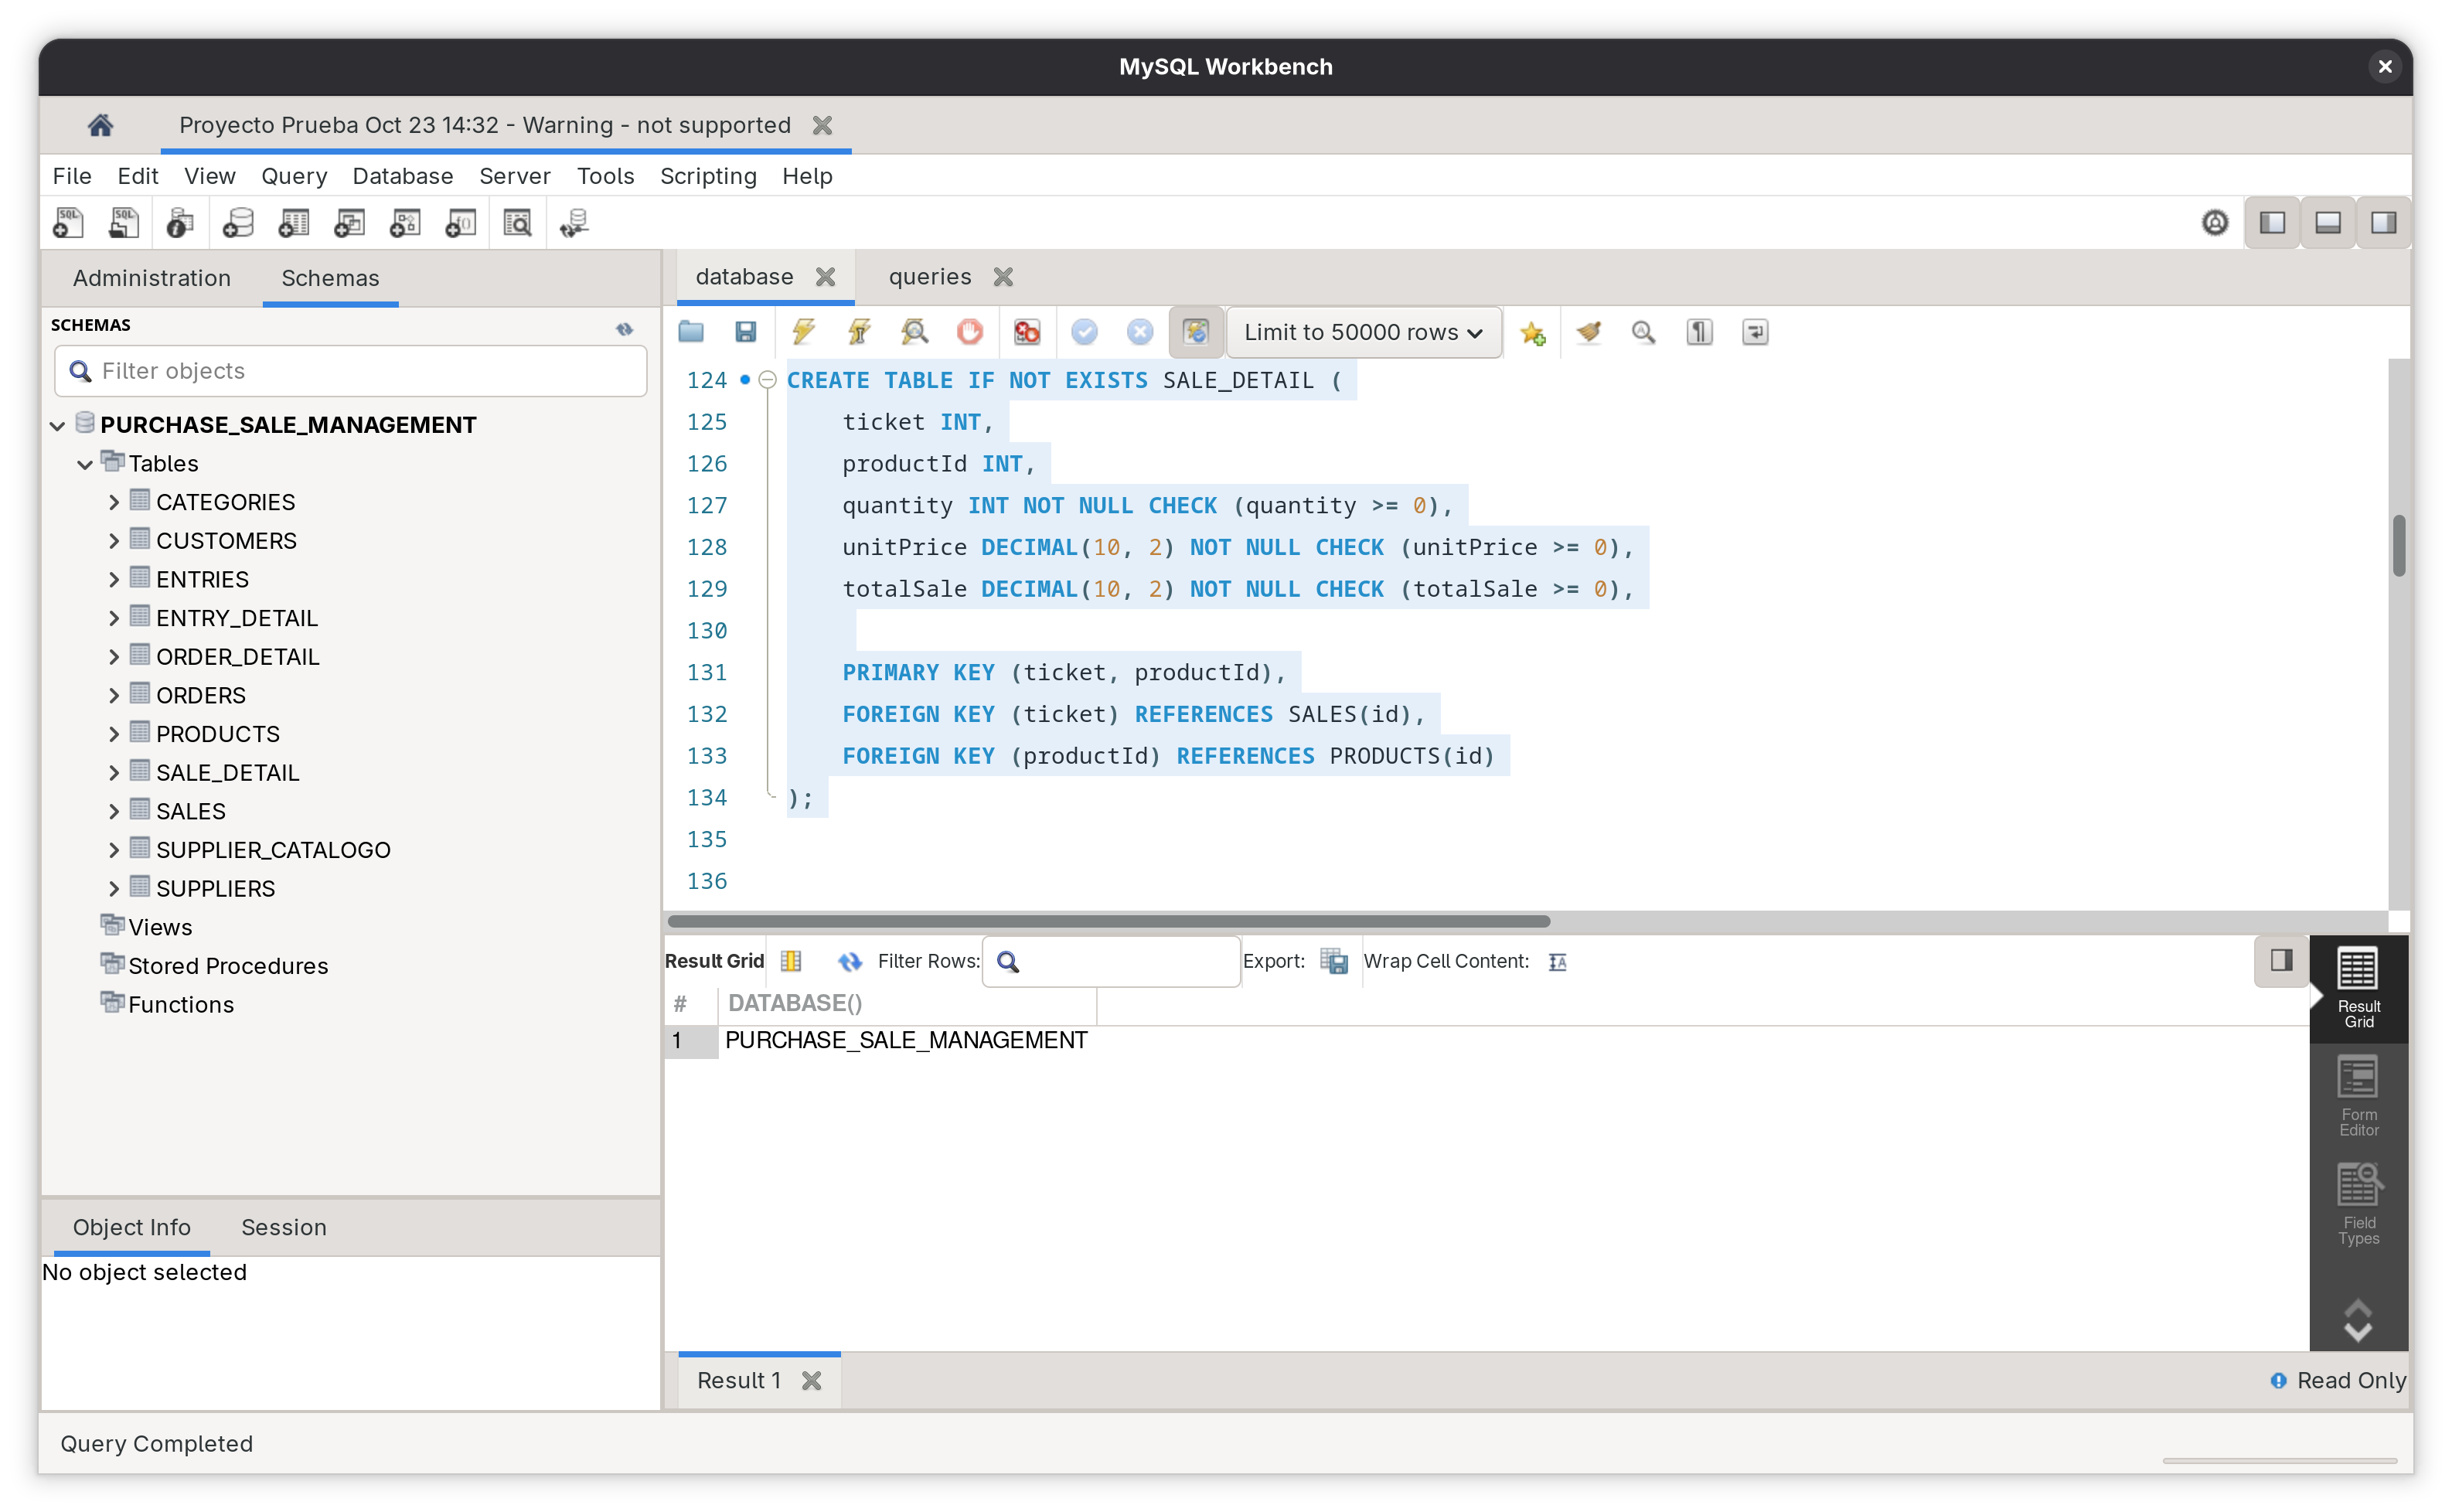
\includegraphics[
        width=0.9\linewidth
        ]{../img/evidencias/pruebas-creacion-db-tablas.png}
	\caption{\textit{Creación de la base de datos y sus tablas}}
	\label{fig:creacion-db-tablas}
\end{figure}

\begin{figure}[!htb]
	\centering
	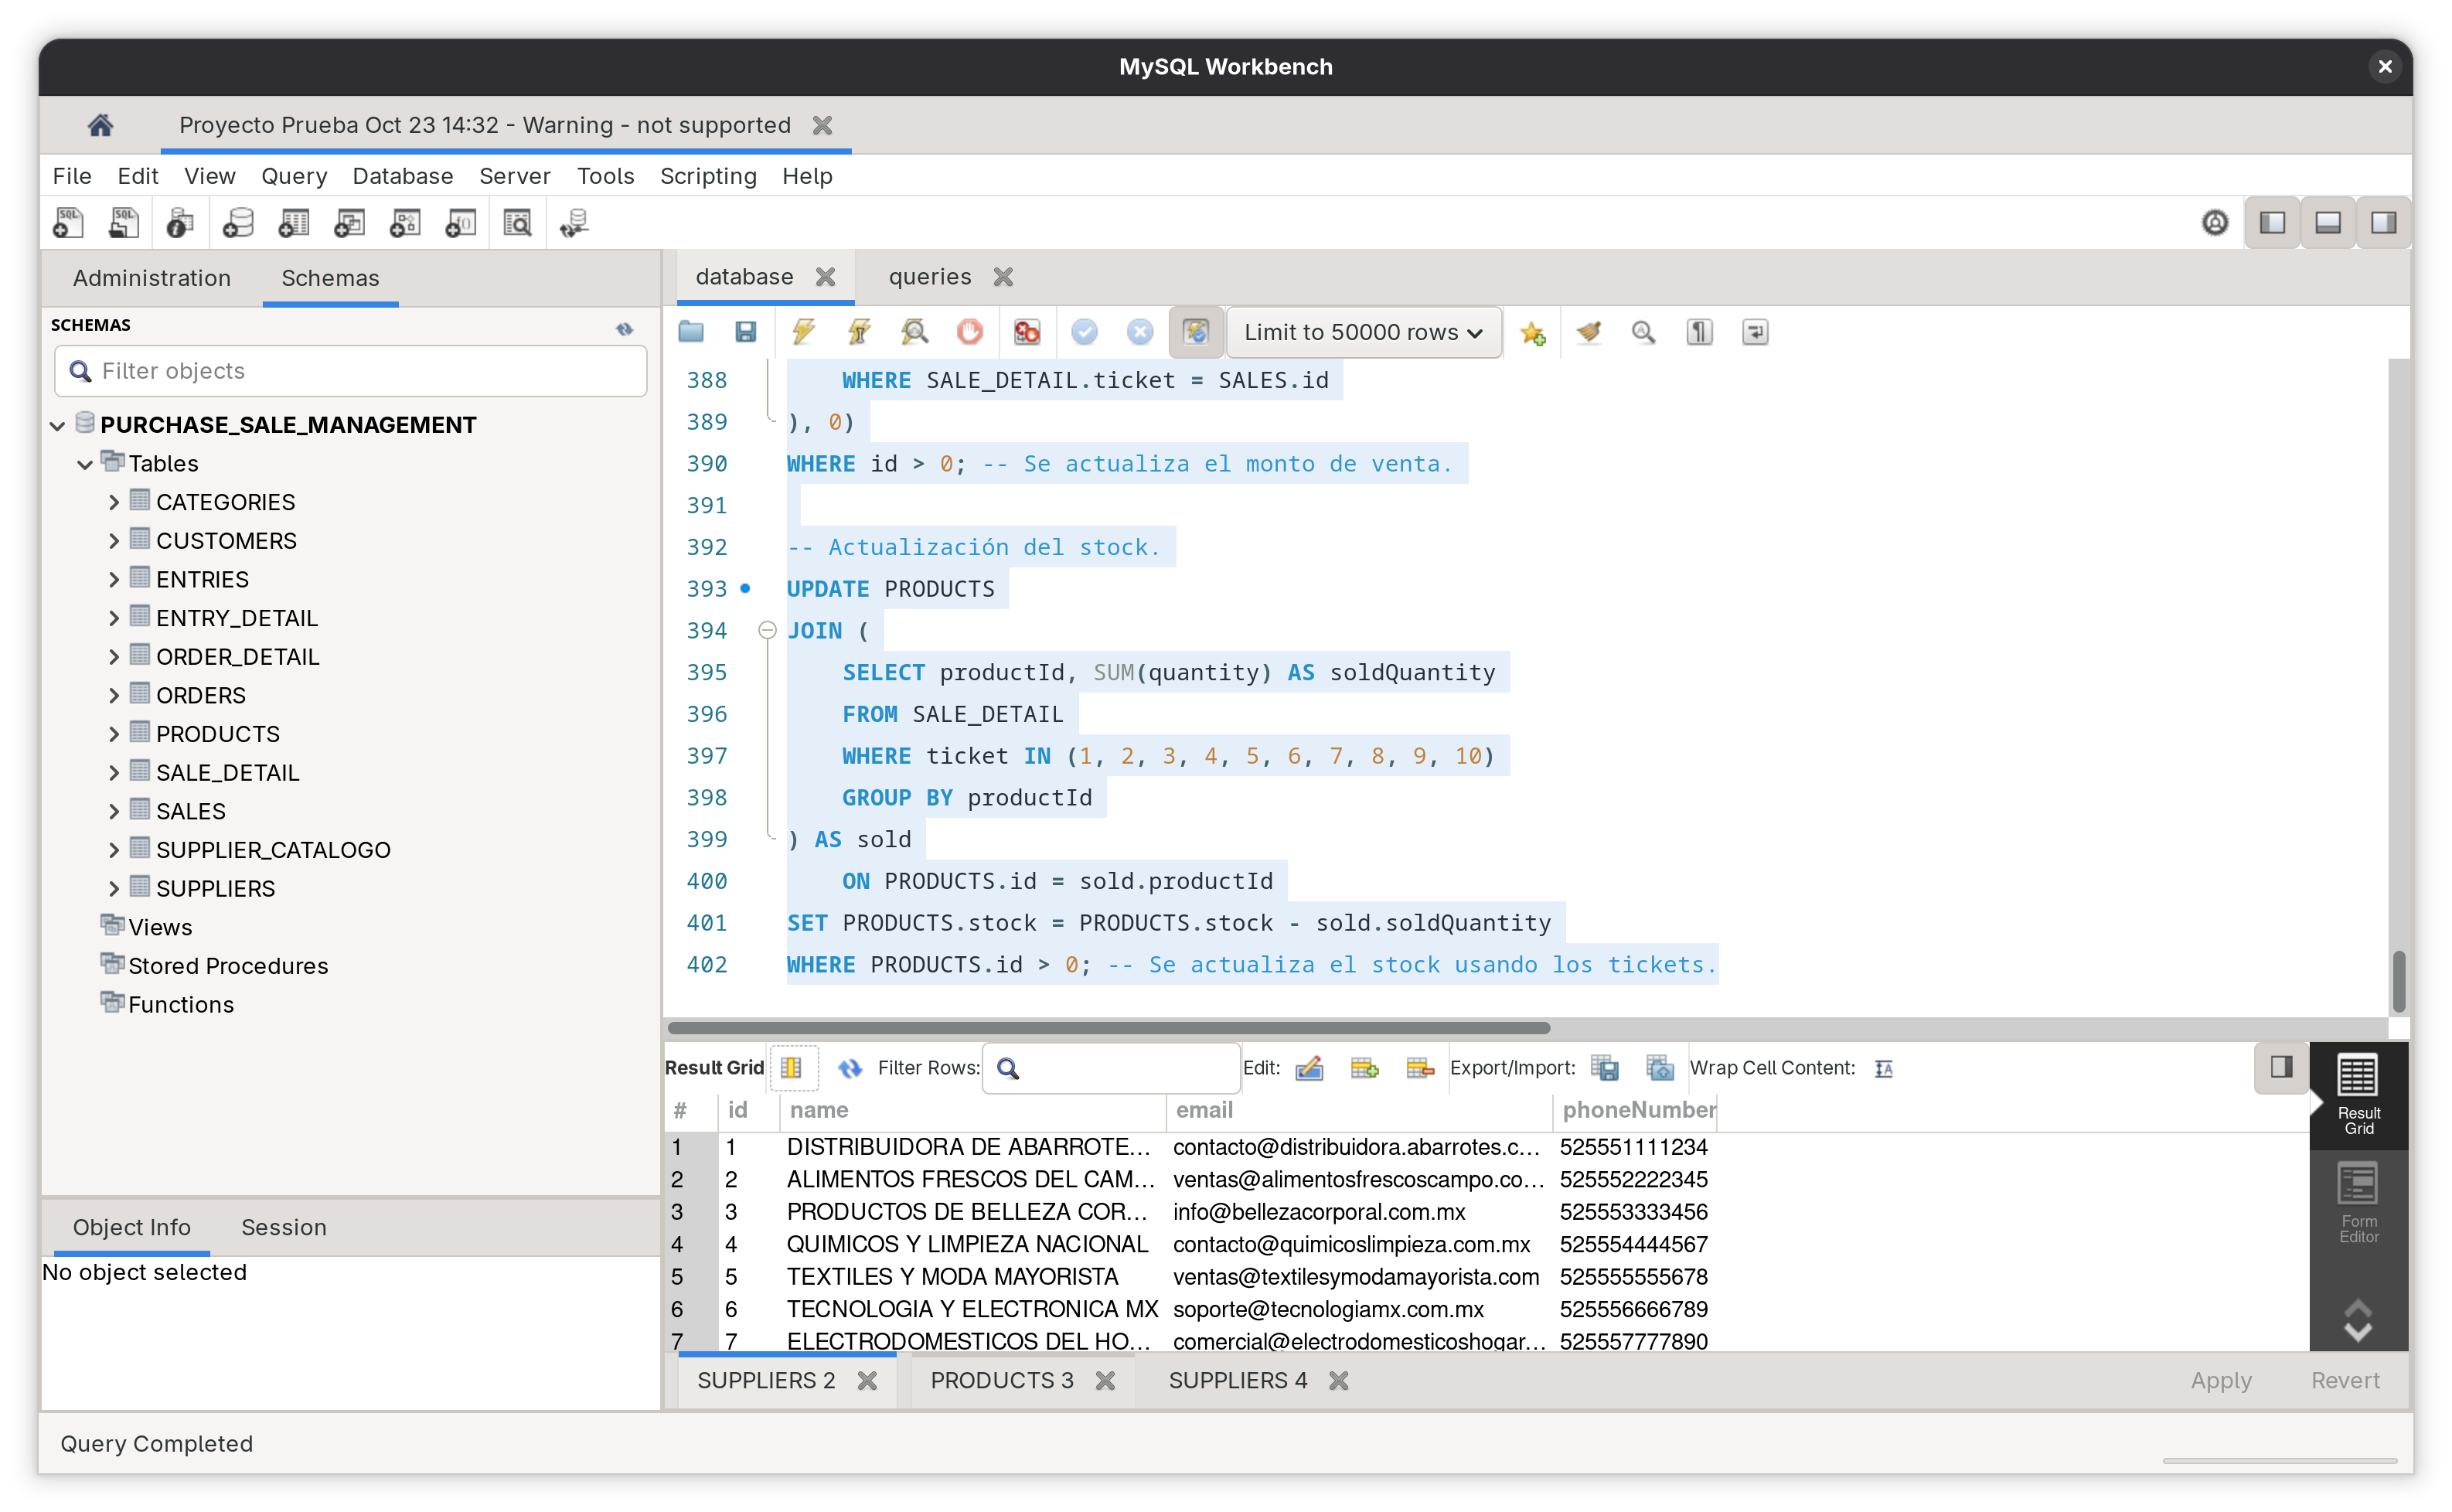
\includegraphics[
        width=0.9\linewidth
        ]{../img/evidencias/pruebas-insercion-datos.png}
	\caption{\textit{Inserción de los primeros datos}}
	\label{fig:insercion-datos}
\end{figure}

\vfill

\begin{figure}[!htb]
	\centering
	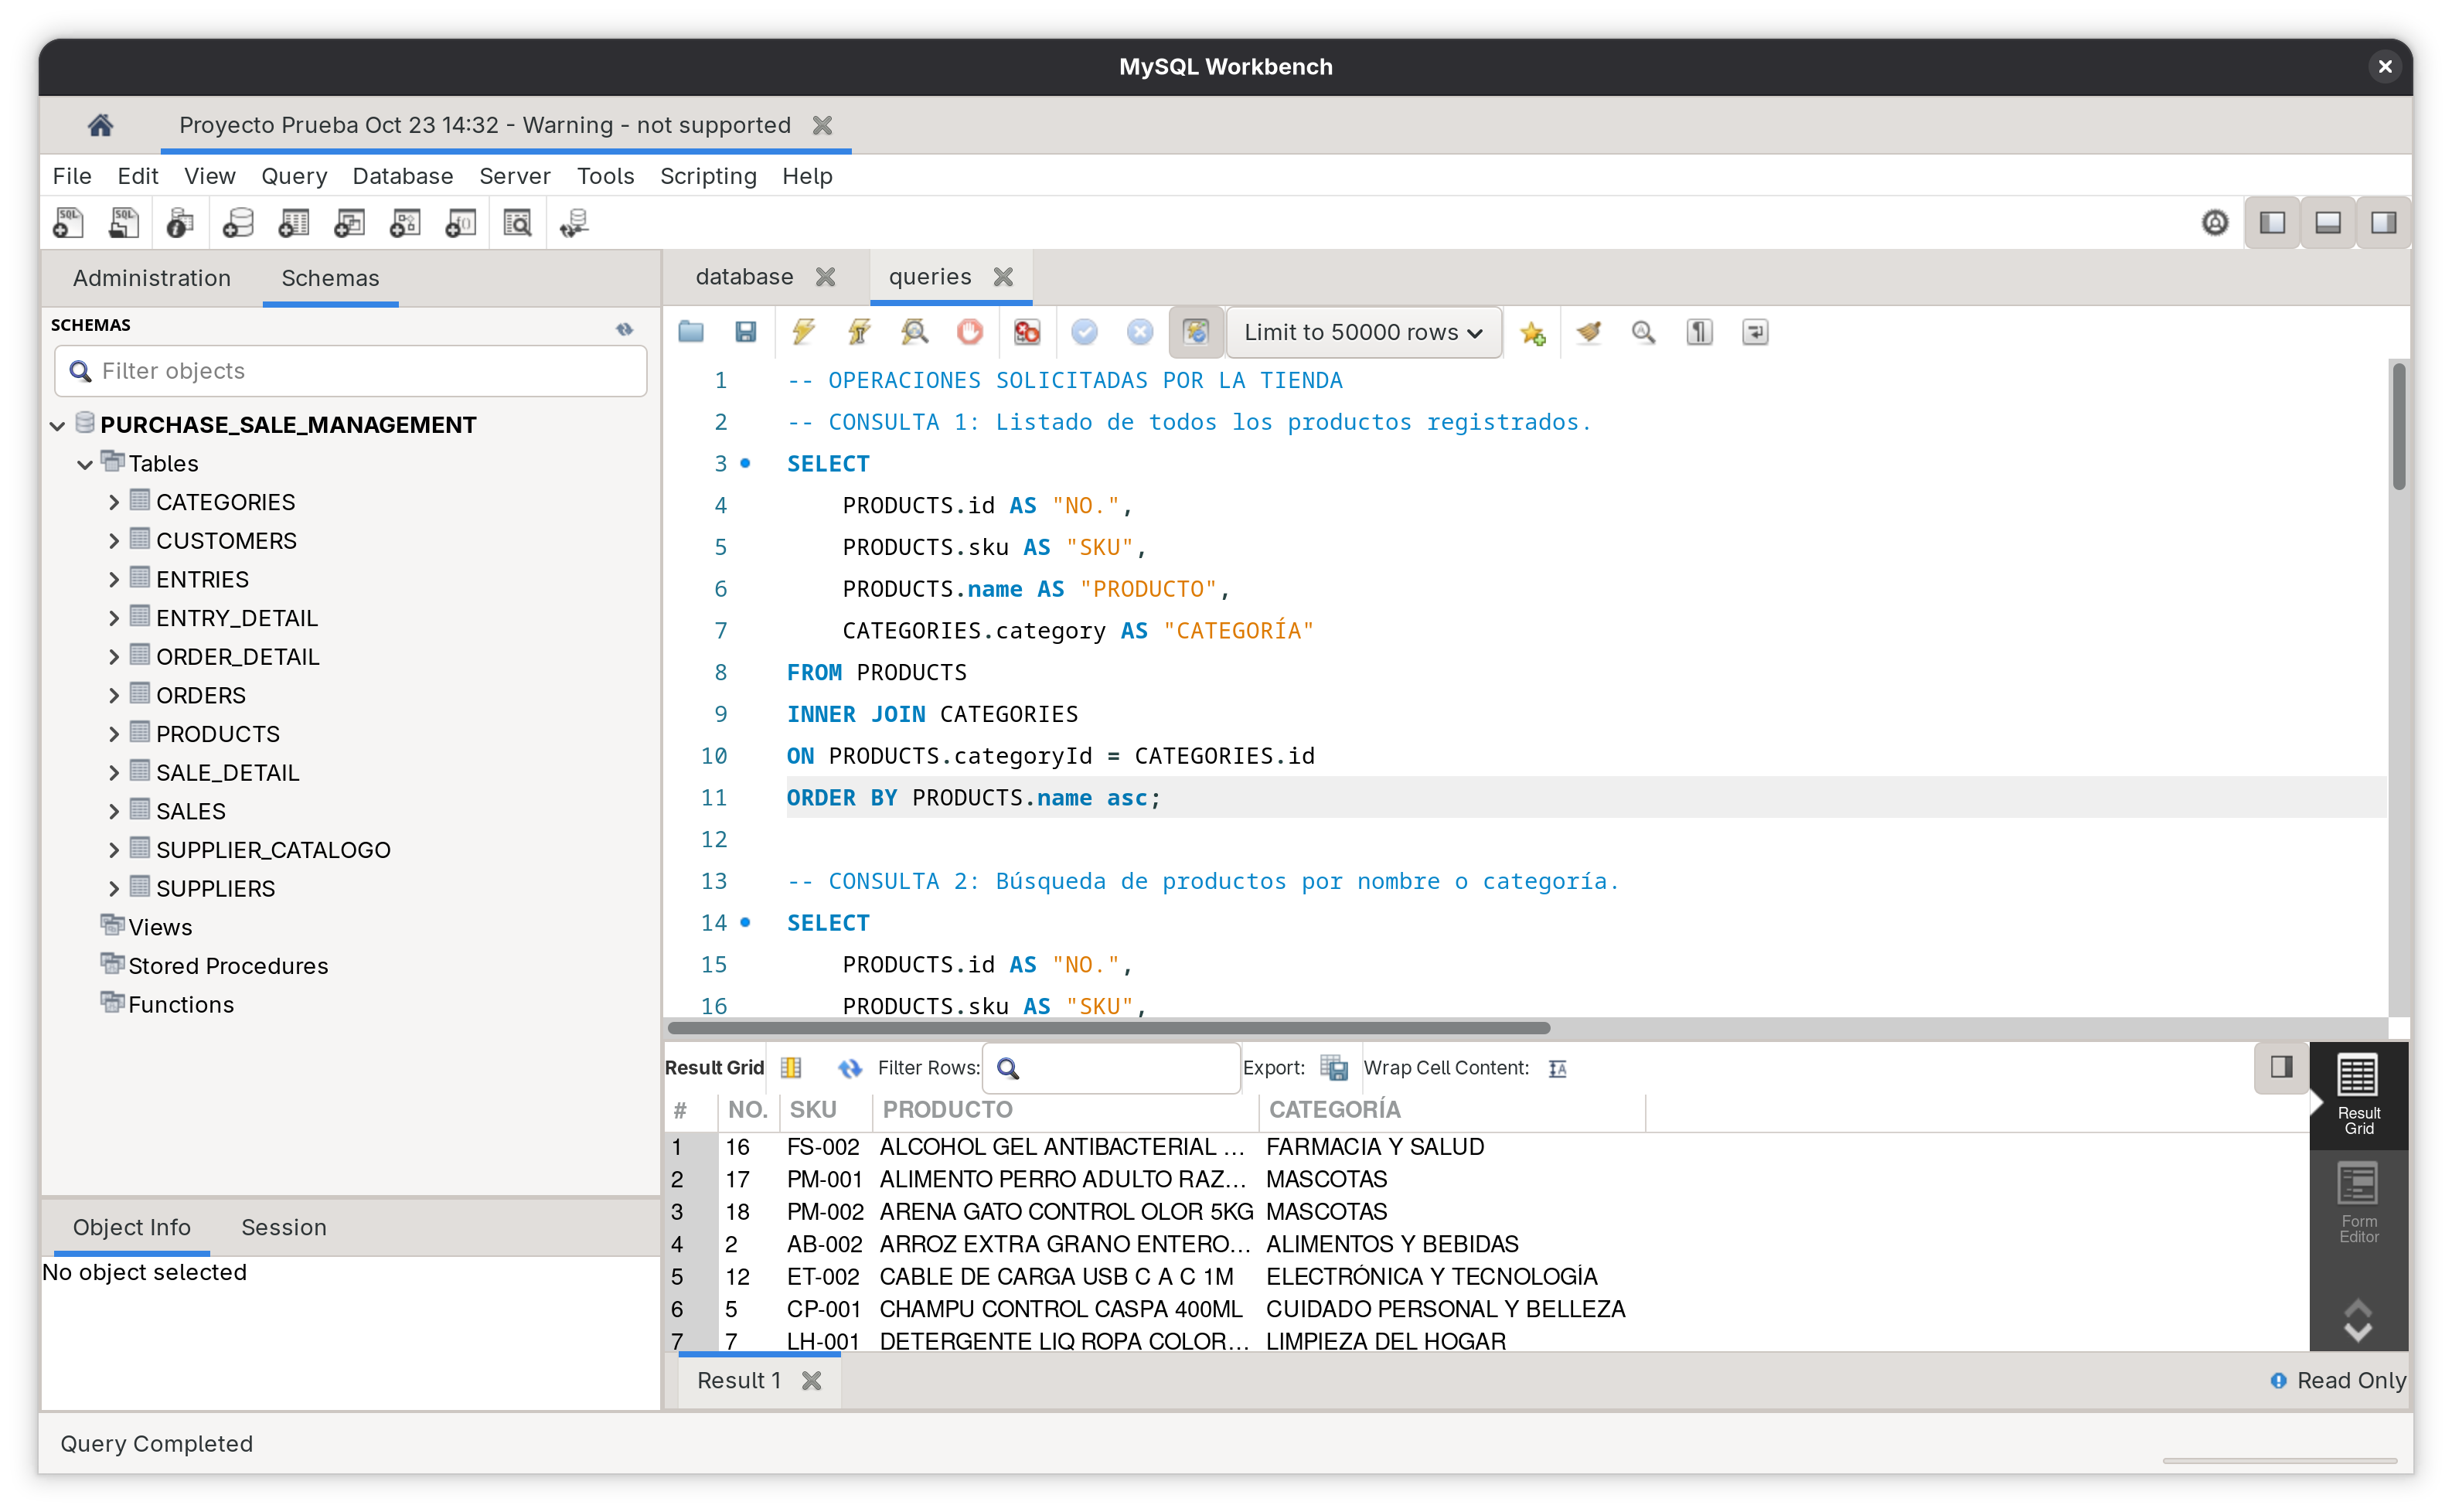
\includegraphics[
        width=0.9\linewidth
        ]{../img/evidencias/pruebas-consulta-1.png}
	\caption{\textit{Consulta 1}}
	\label{fig:consulta-}
\end{figure}

\begin{figure}[!htb]
	\centering
	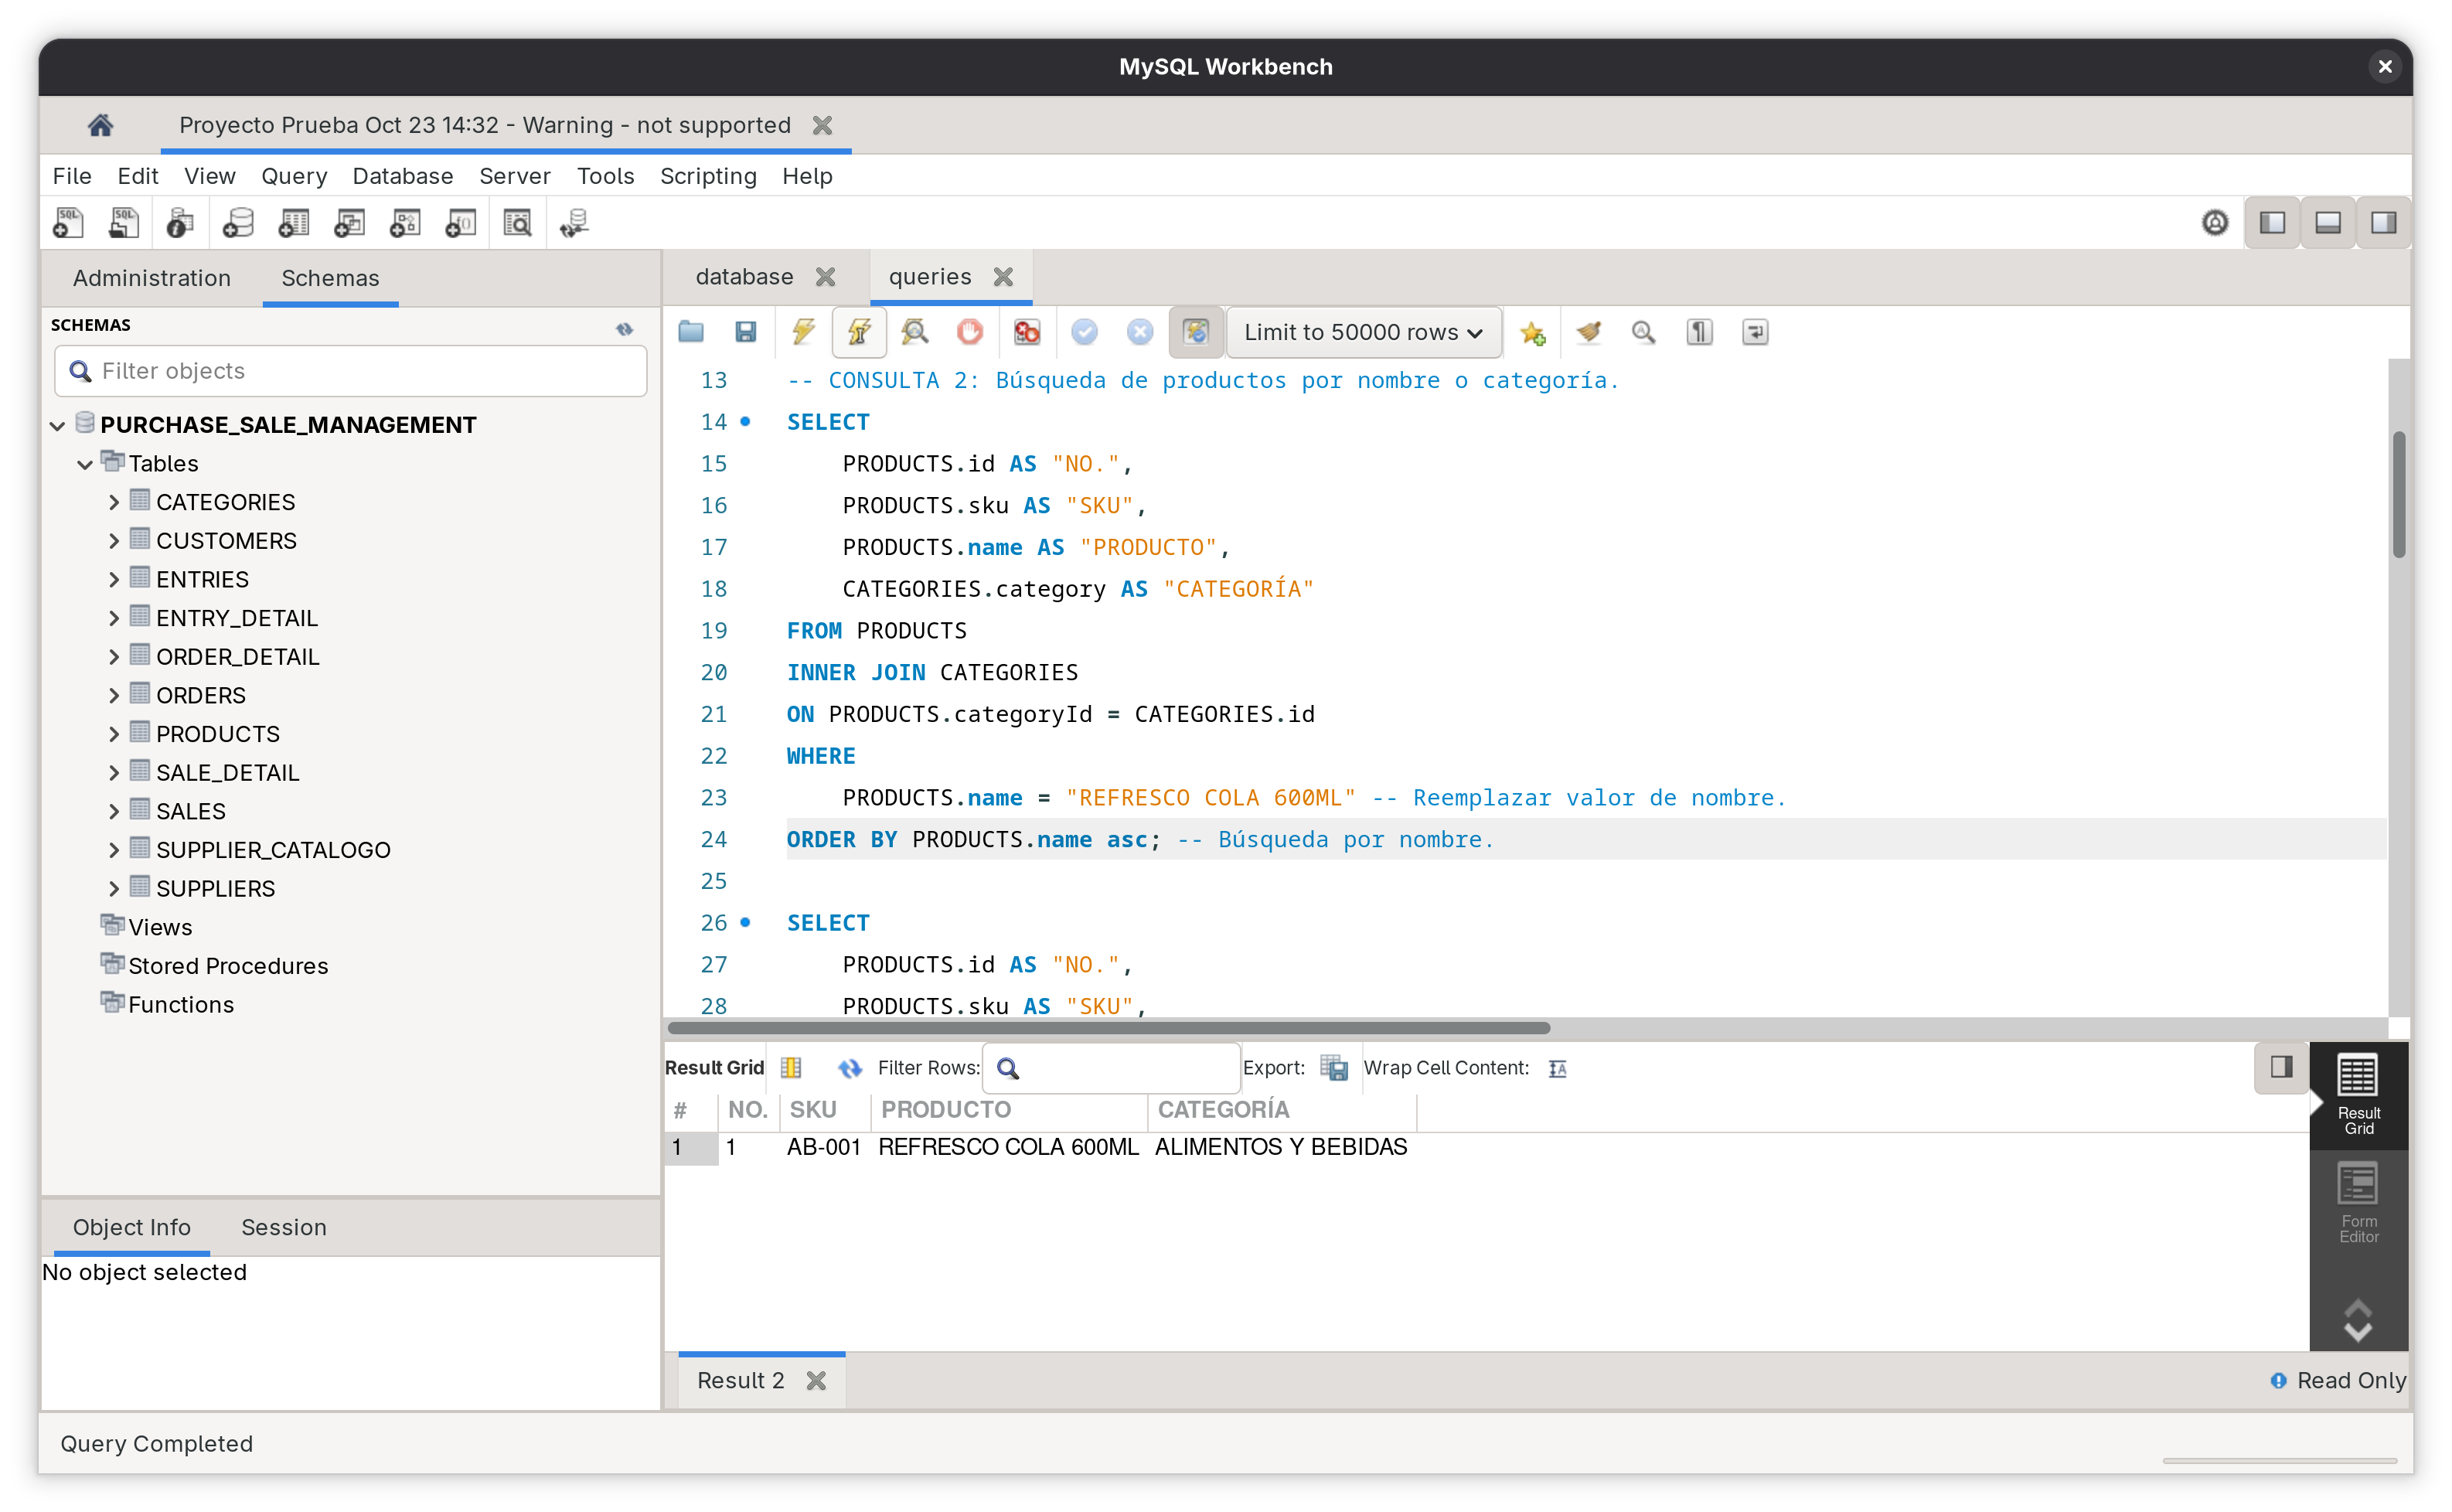
\includegraphics[
        width=0.9\linewidth
        ]{../img/evidencias/pruebas-consulta-2.png}
	\caption{\textit{Consulta 2}}
	\label{fig:consulta-2}
\end{figure}

\begin{figure}[!htb]
	\centering
	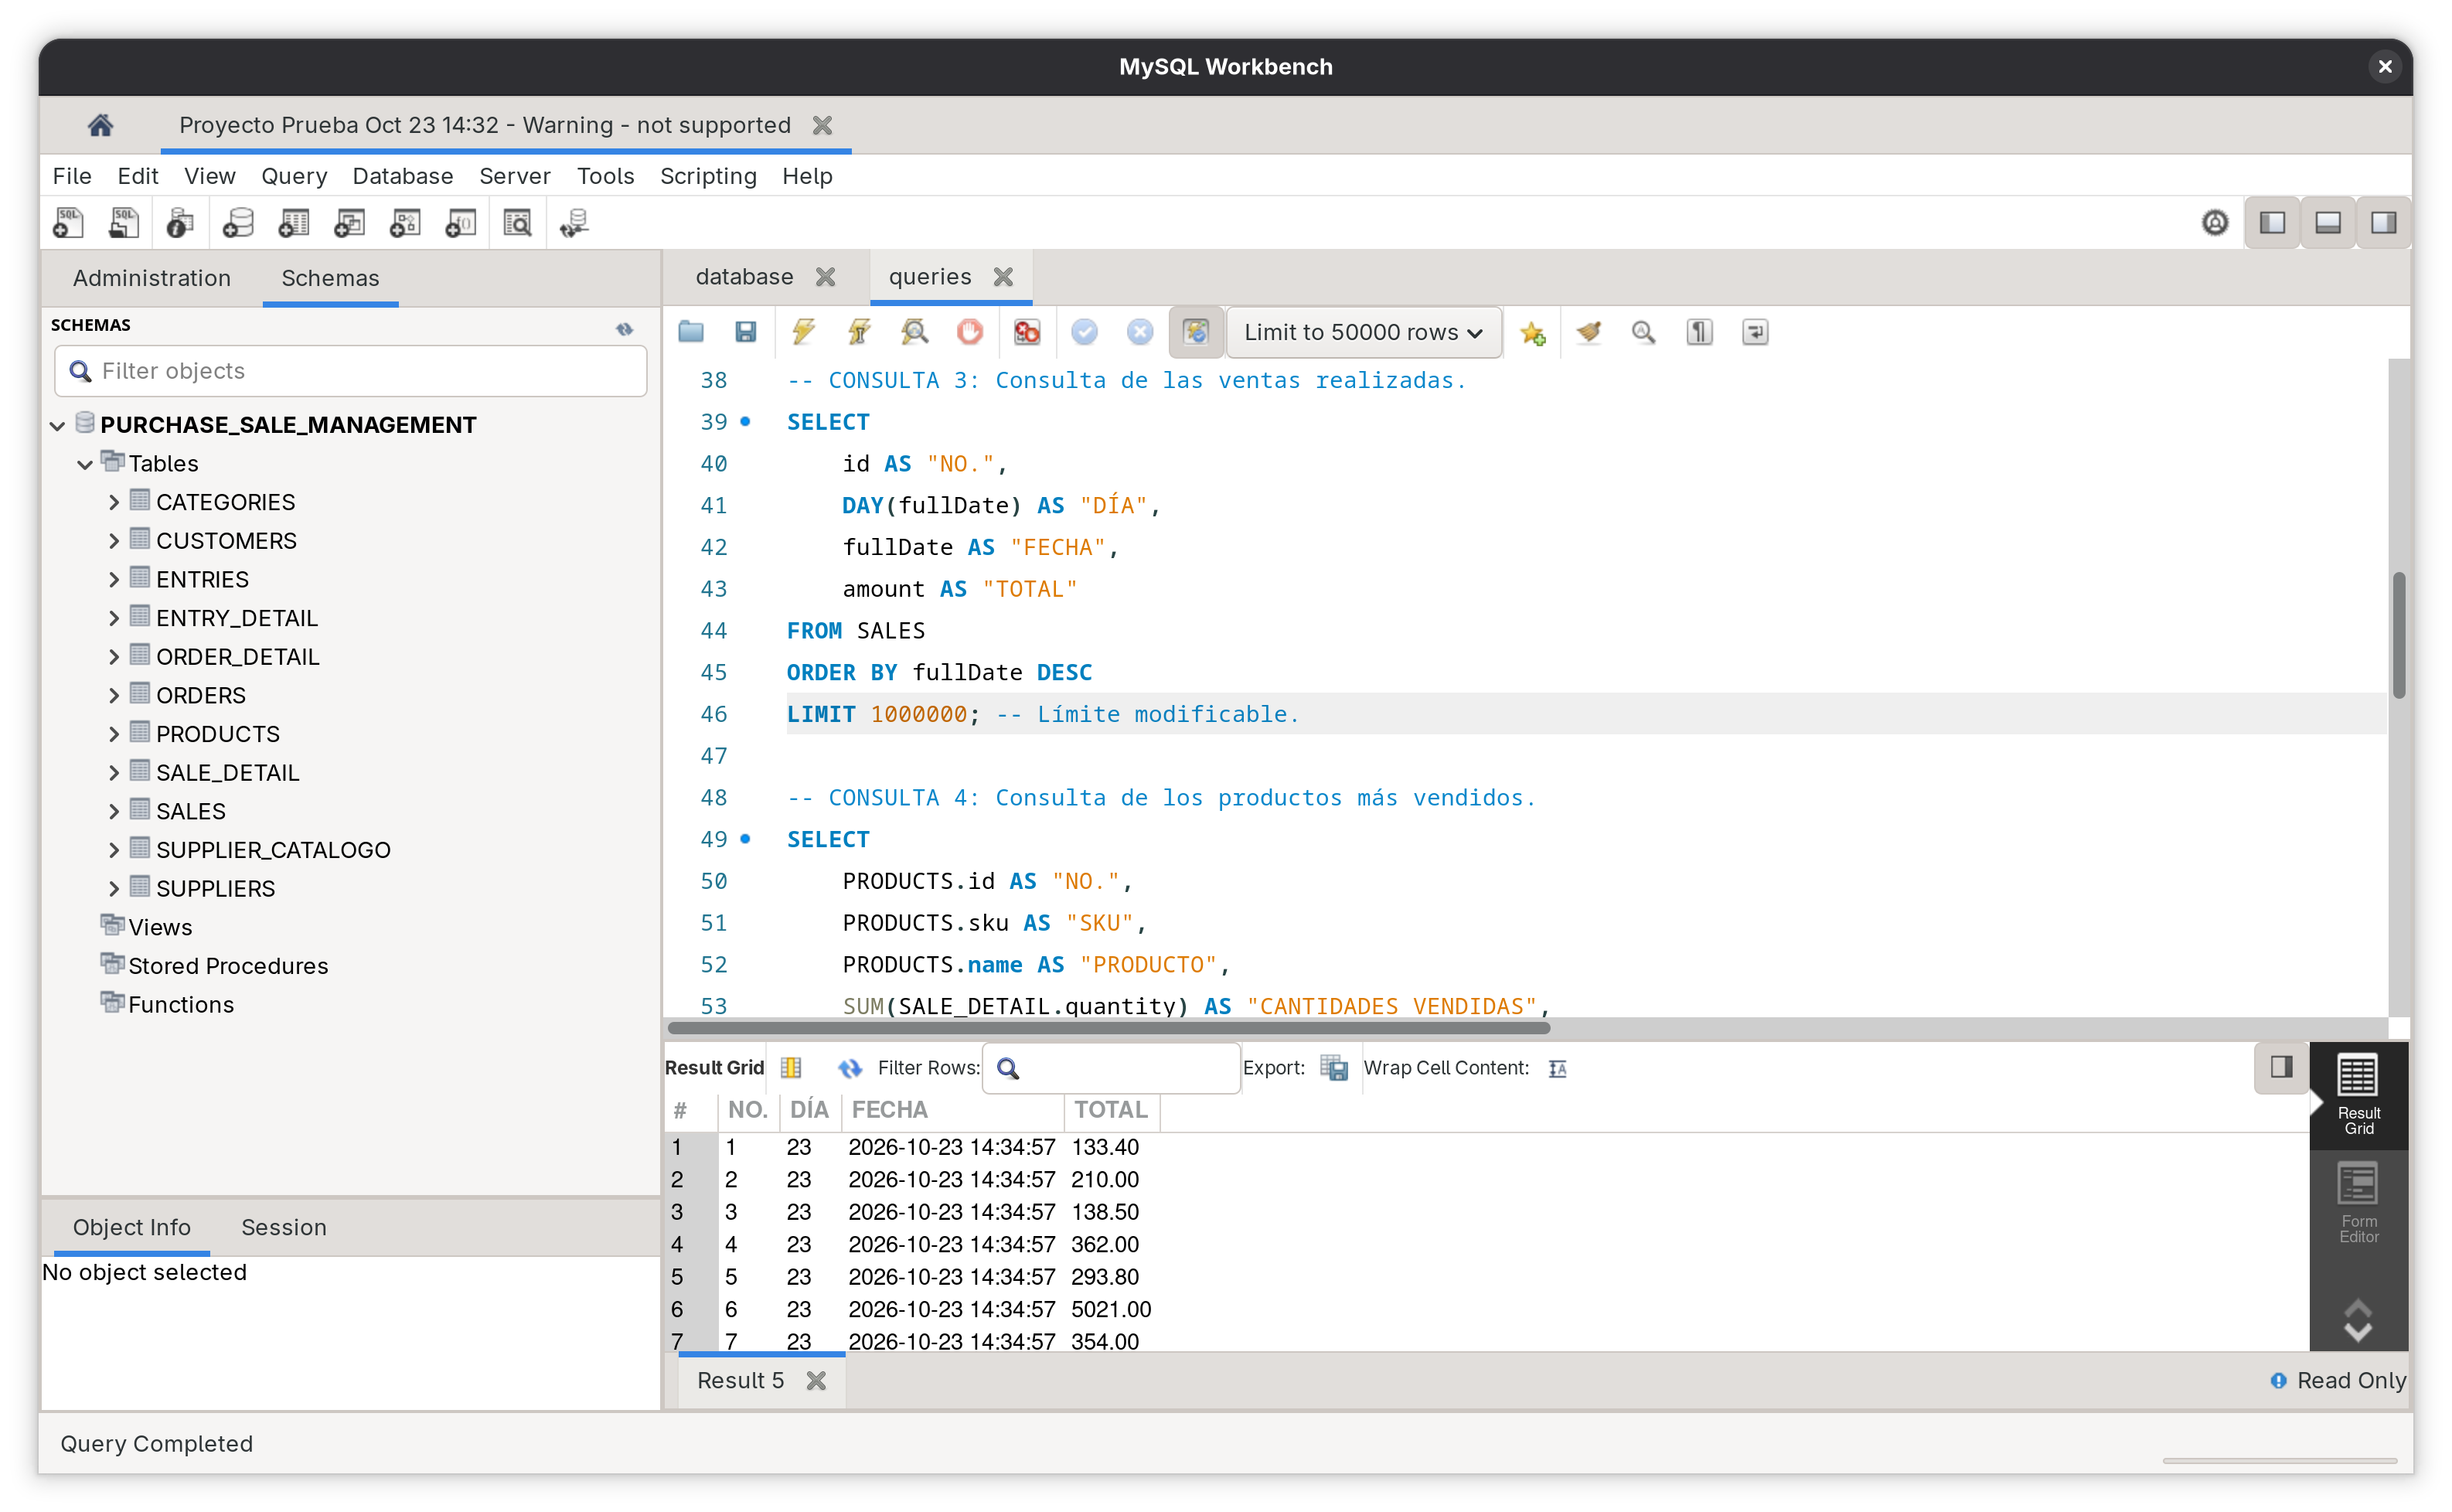
\includegraphics[
        width=0.9\linewidth
        ]{../img/evidencias/pruebas-consulta-3.png}
	\caption{\textit{Consulta 3}}
	\label{fig:consulta-3}
\end{figure}

\begin{figure}[!htb]
	\centering
	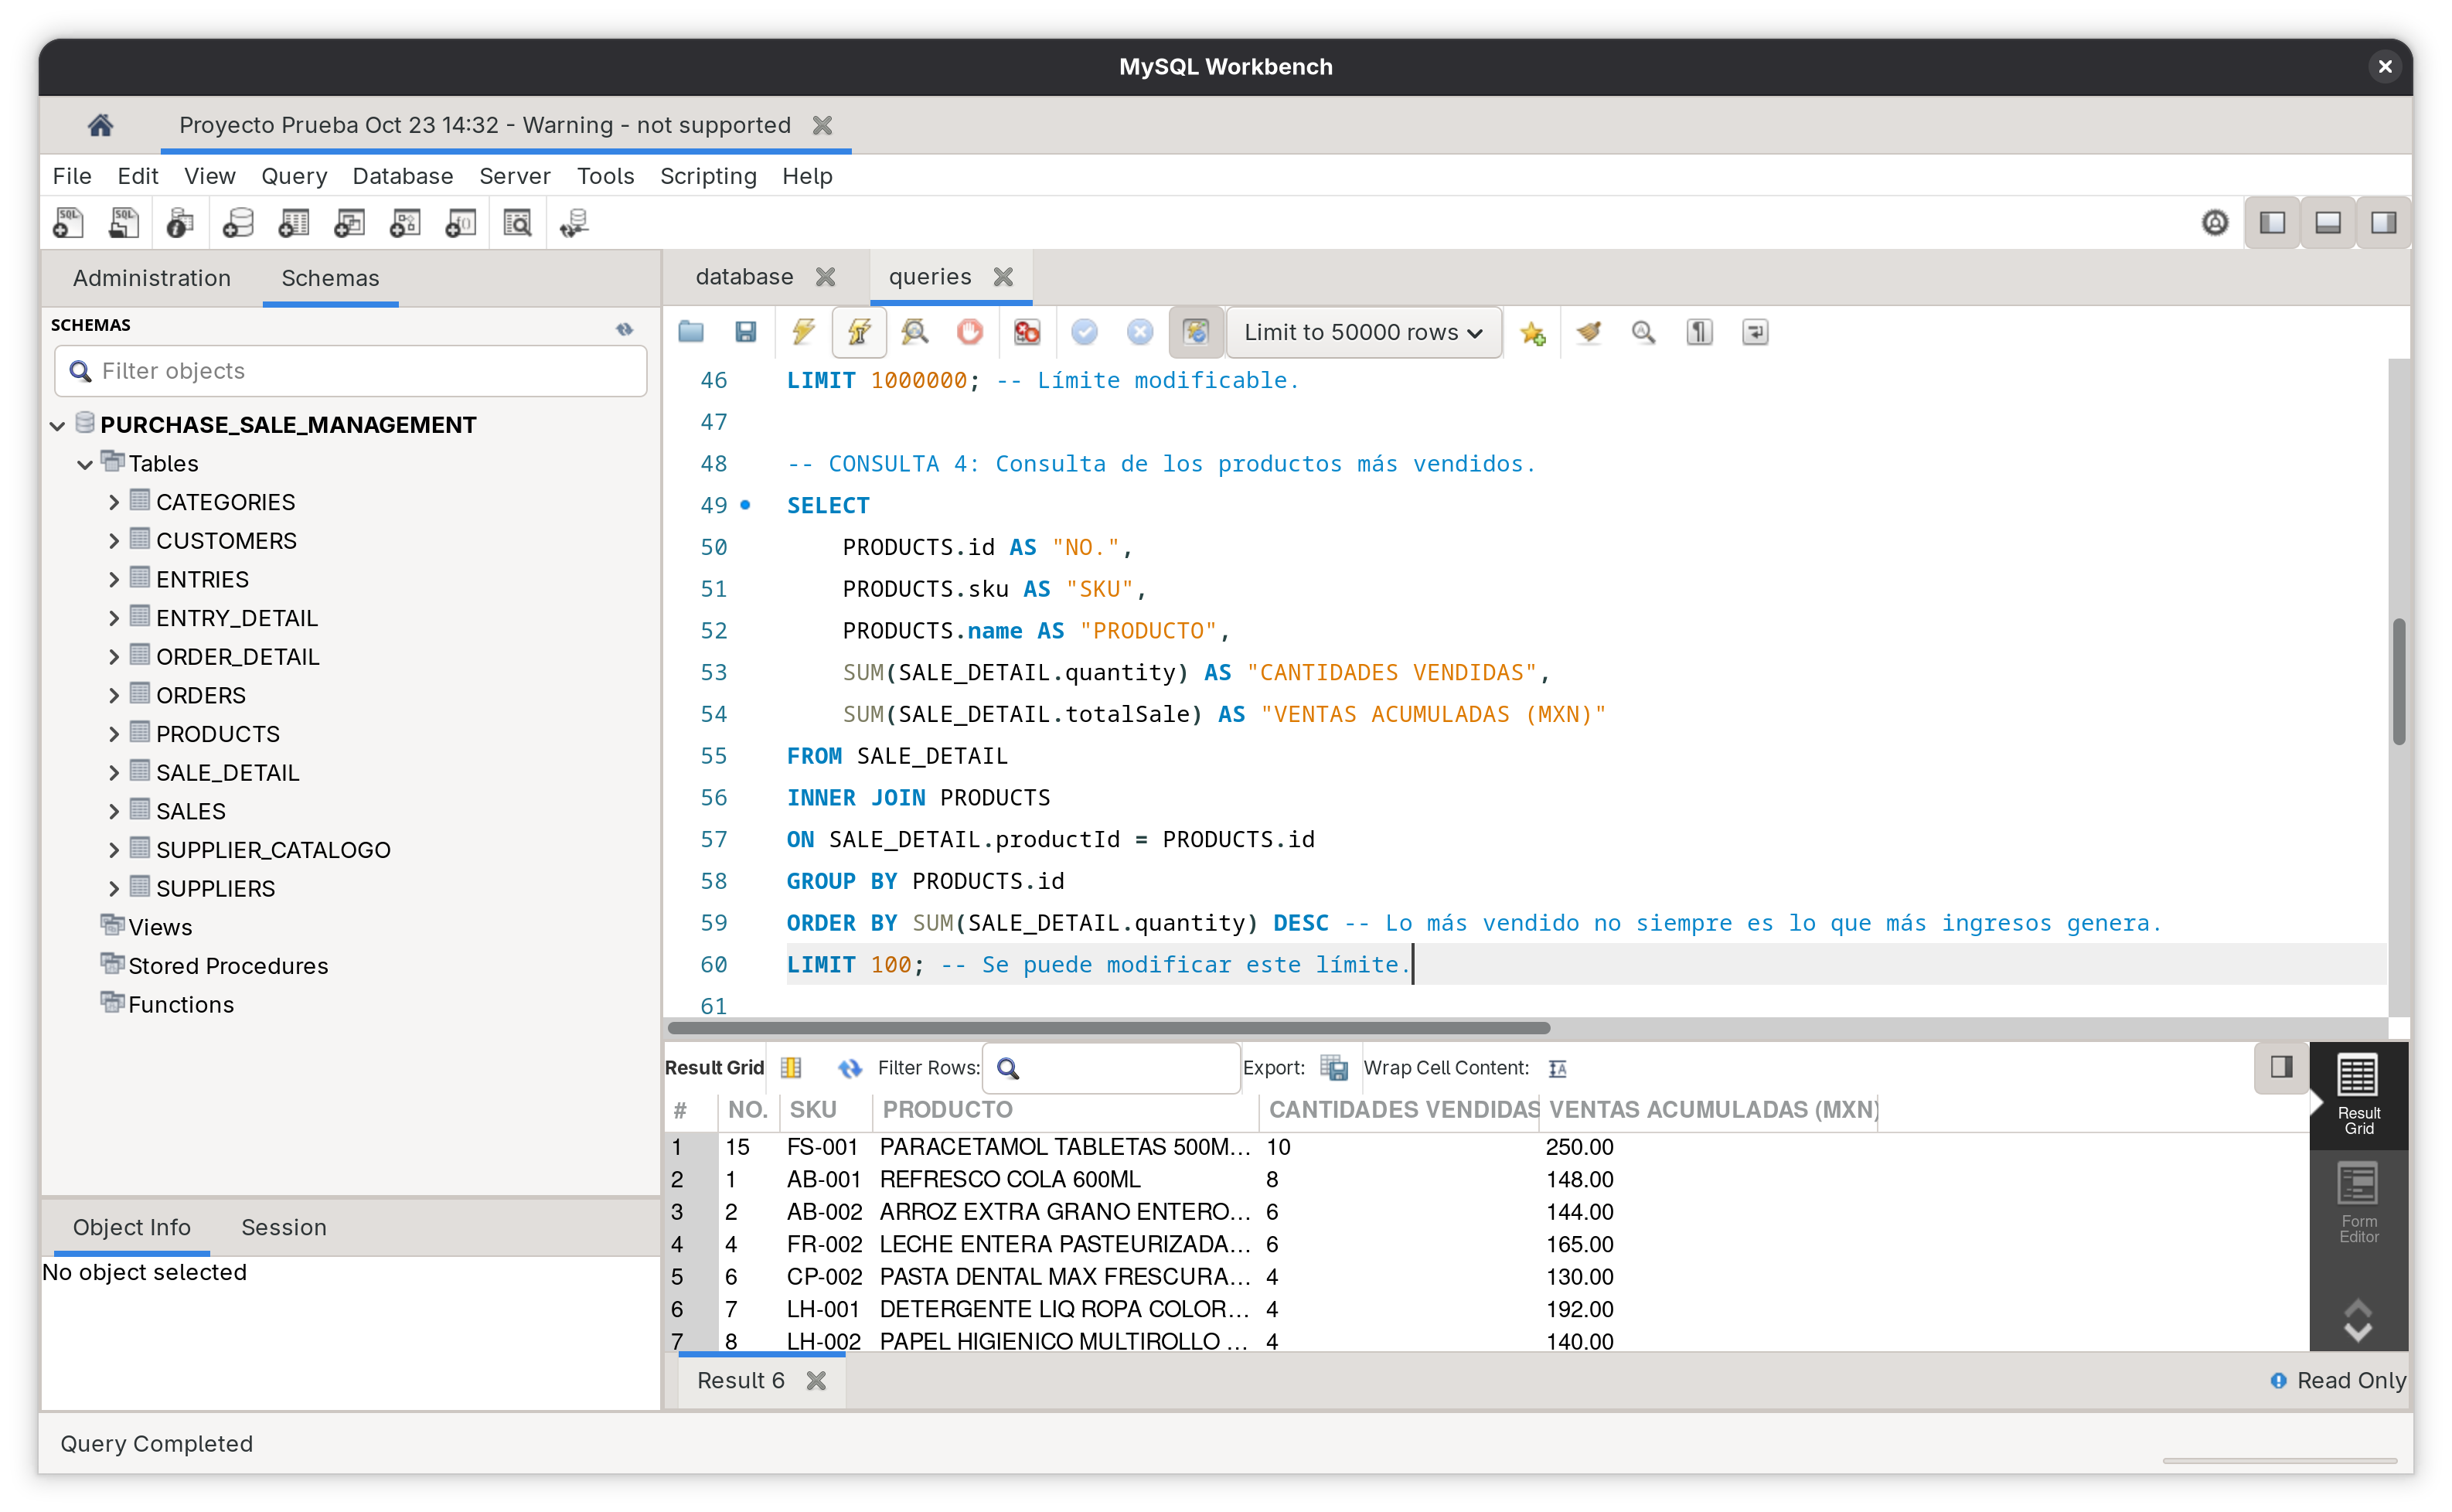
\includegraphics[
        width=0.9\linewidth
        ]{../img/evidencias/pruebas-consulta-4.png}
	\caption{\textit{Consulta 4}}
	\label{fig:consulta-4}
\end{figure}

\begin{figure}[!htb]
	\centering
	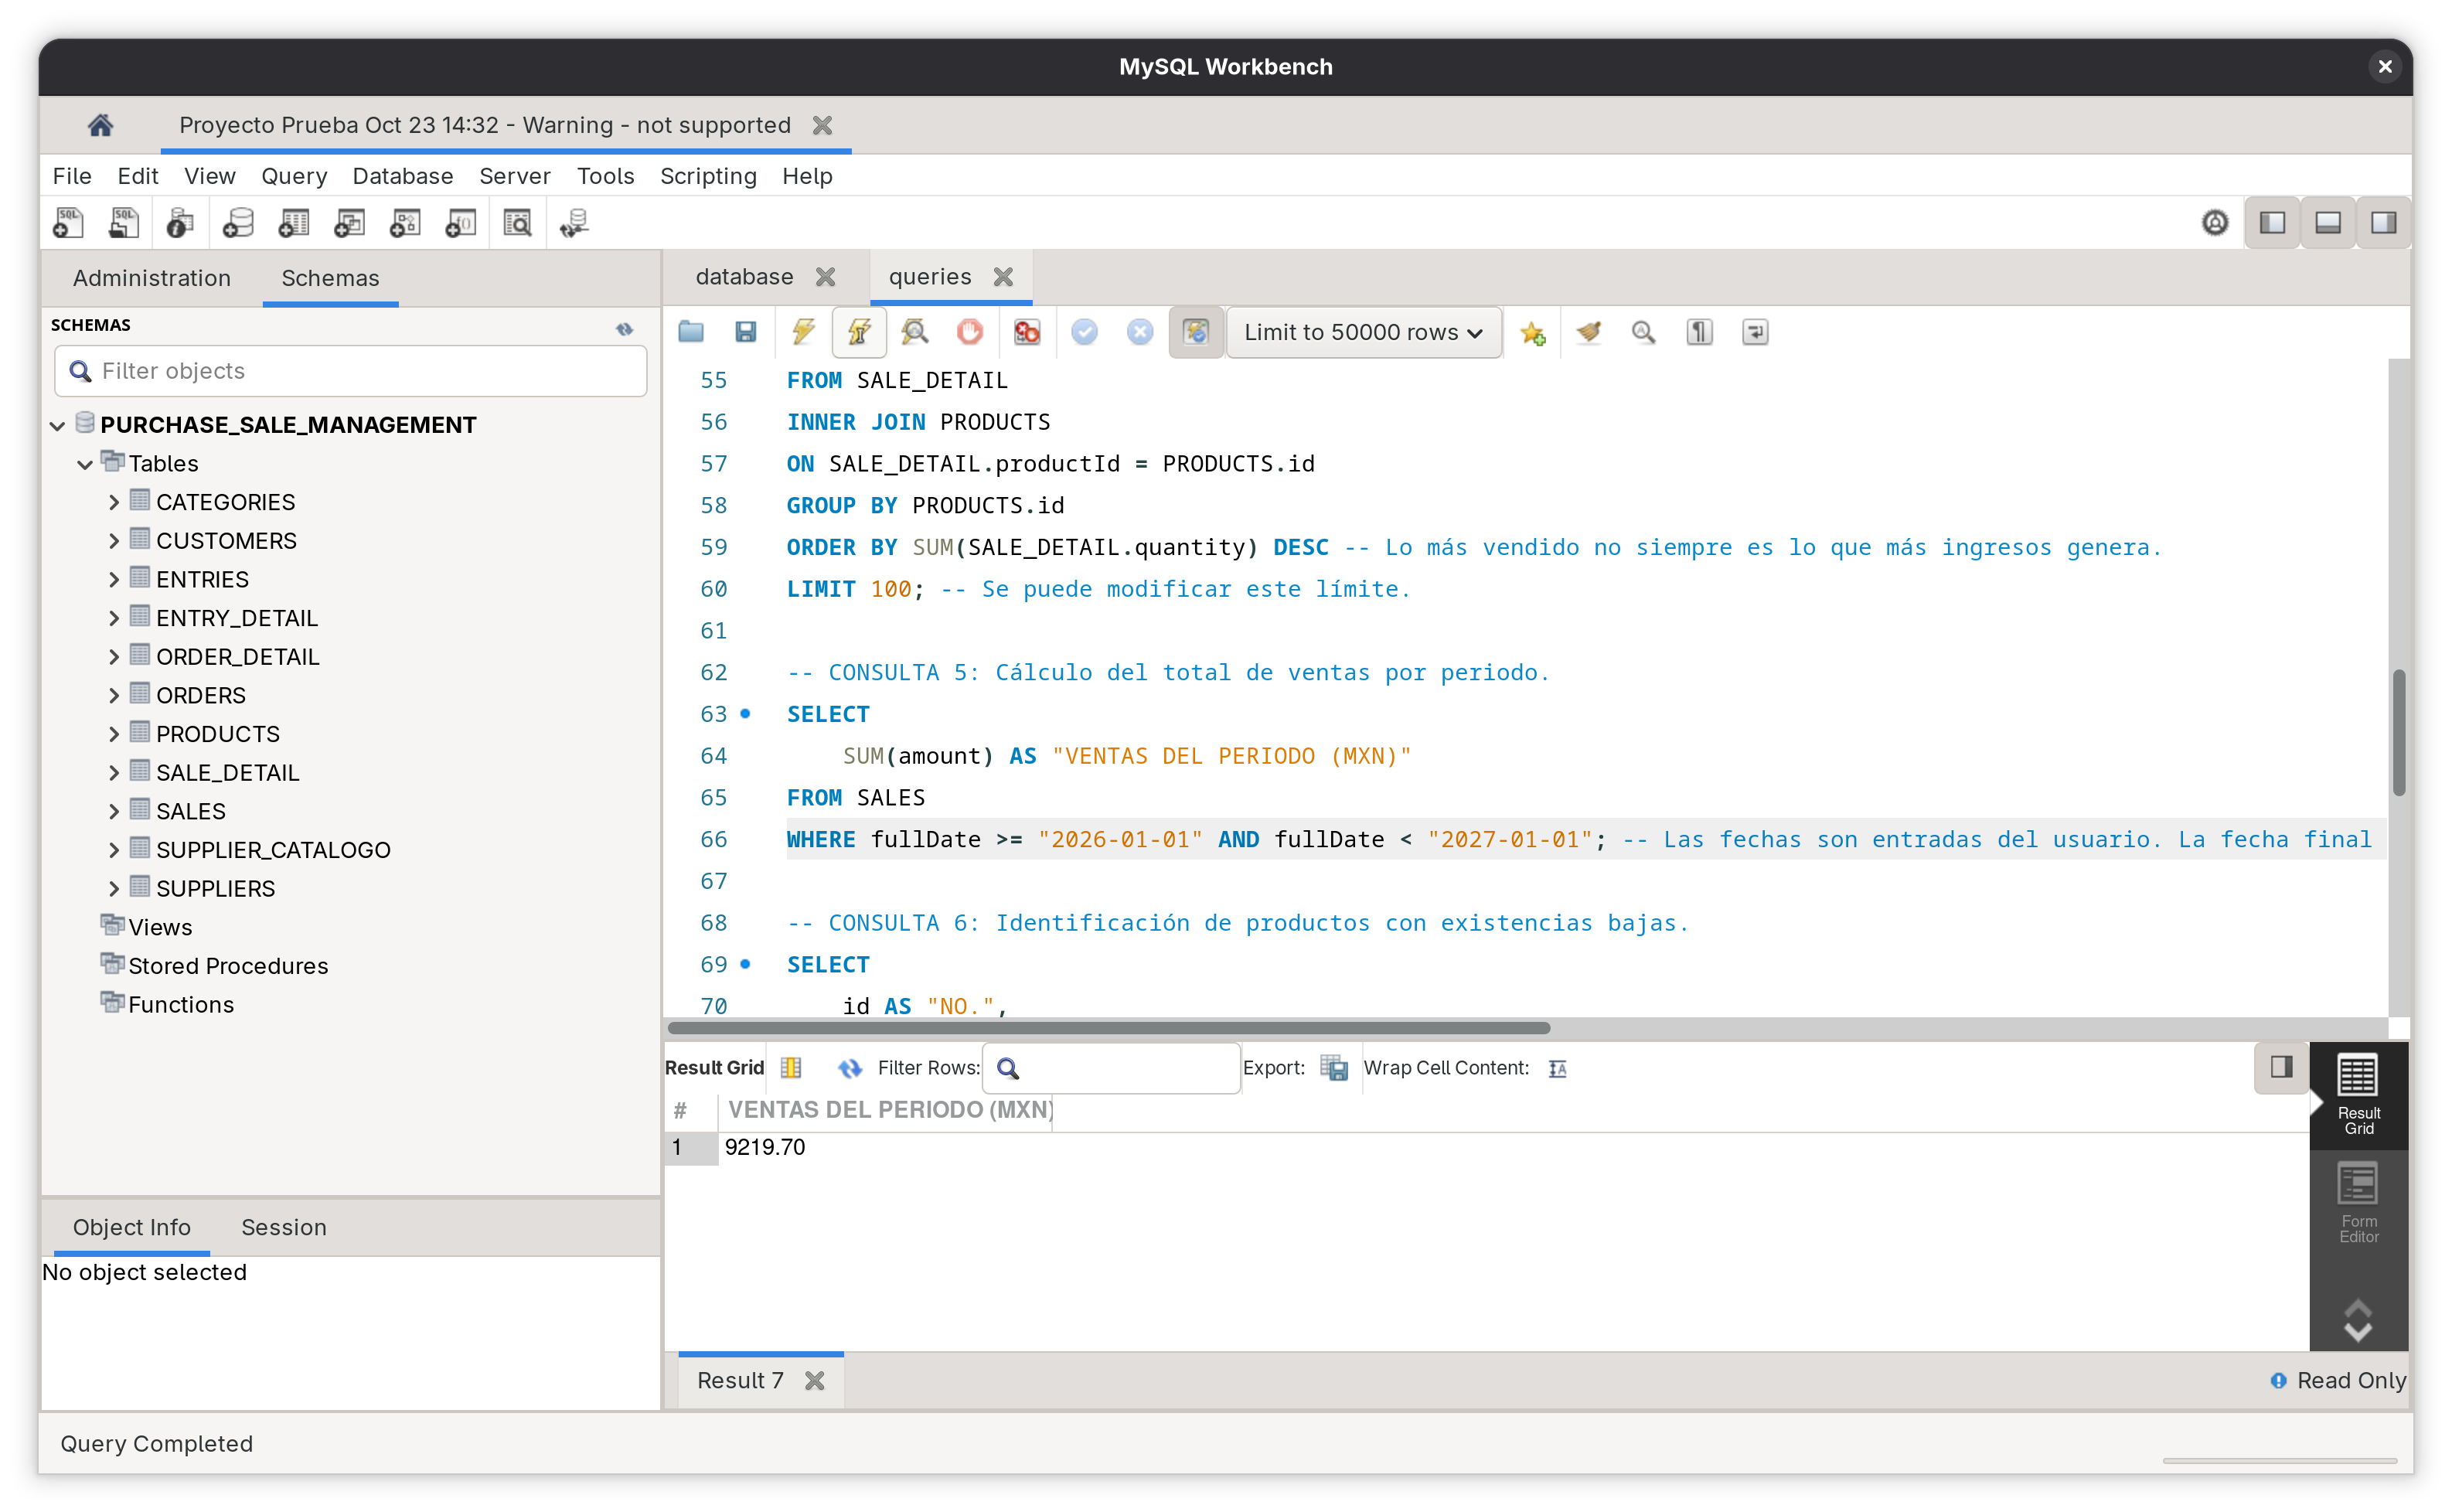
\includegraphics[
        width=0.9\linewidth
        ]{../img/evidencias/pruebas-consulta-5.png}
	\caption{\textit{Consulta 5}}
	\label{fig:consulta-5}
\end{figure}

\begin{figure}[!htb]
	\centering
	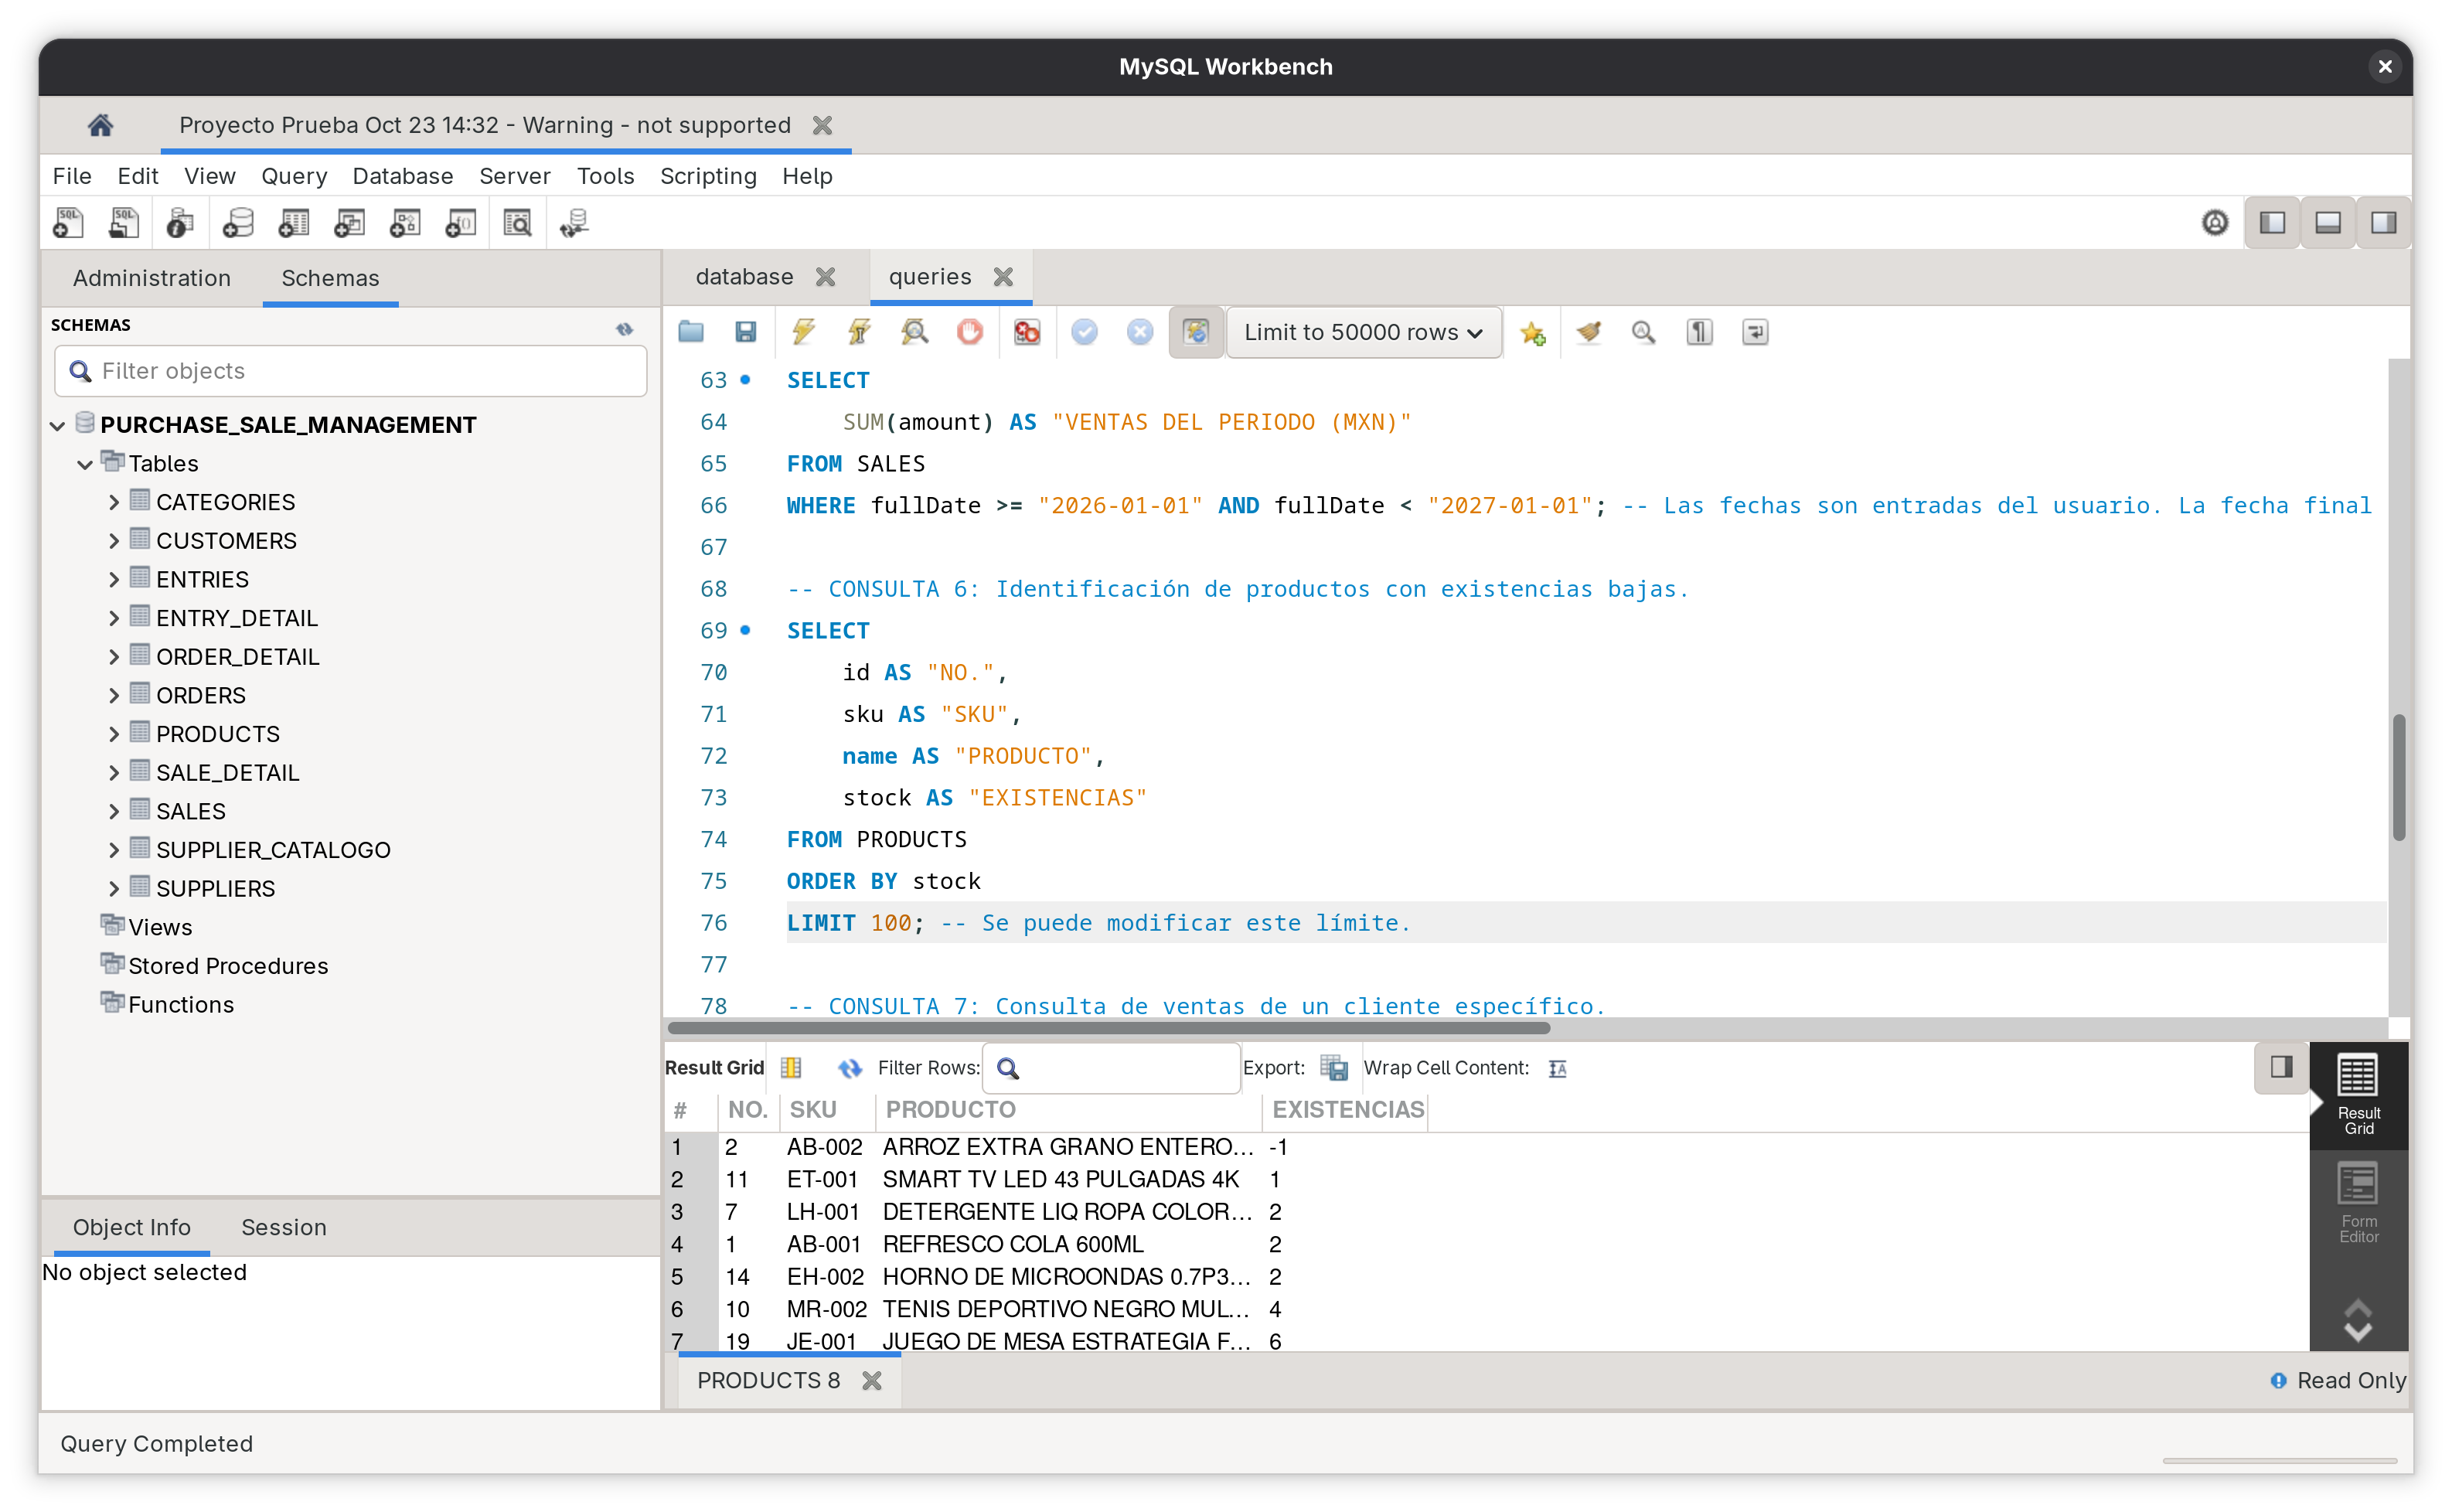
\includegraphics[
        width=0.9\linewidth
        ]{../img/evidencias/pruebas-consulta-6.png}
	\caption{\textit{Consulta 6}}
	\label{fig:consulta-6}
\end{figure}

\begin{figure}[!htb]
	\centering
	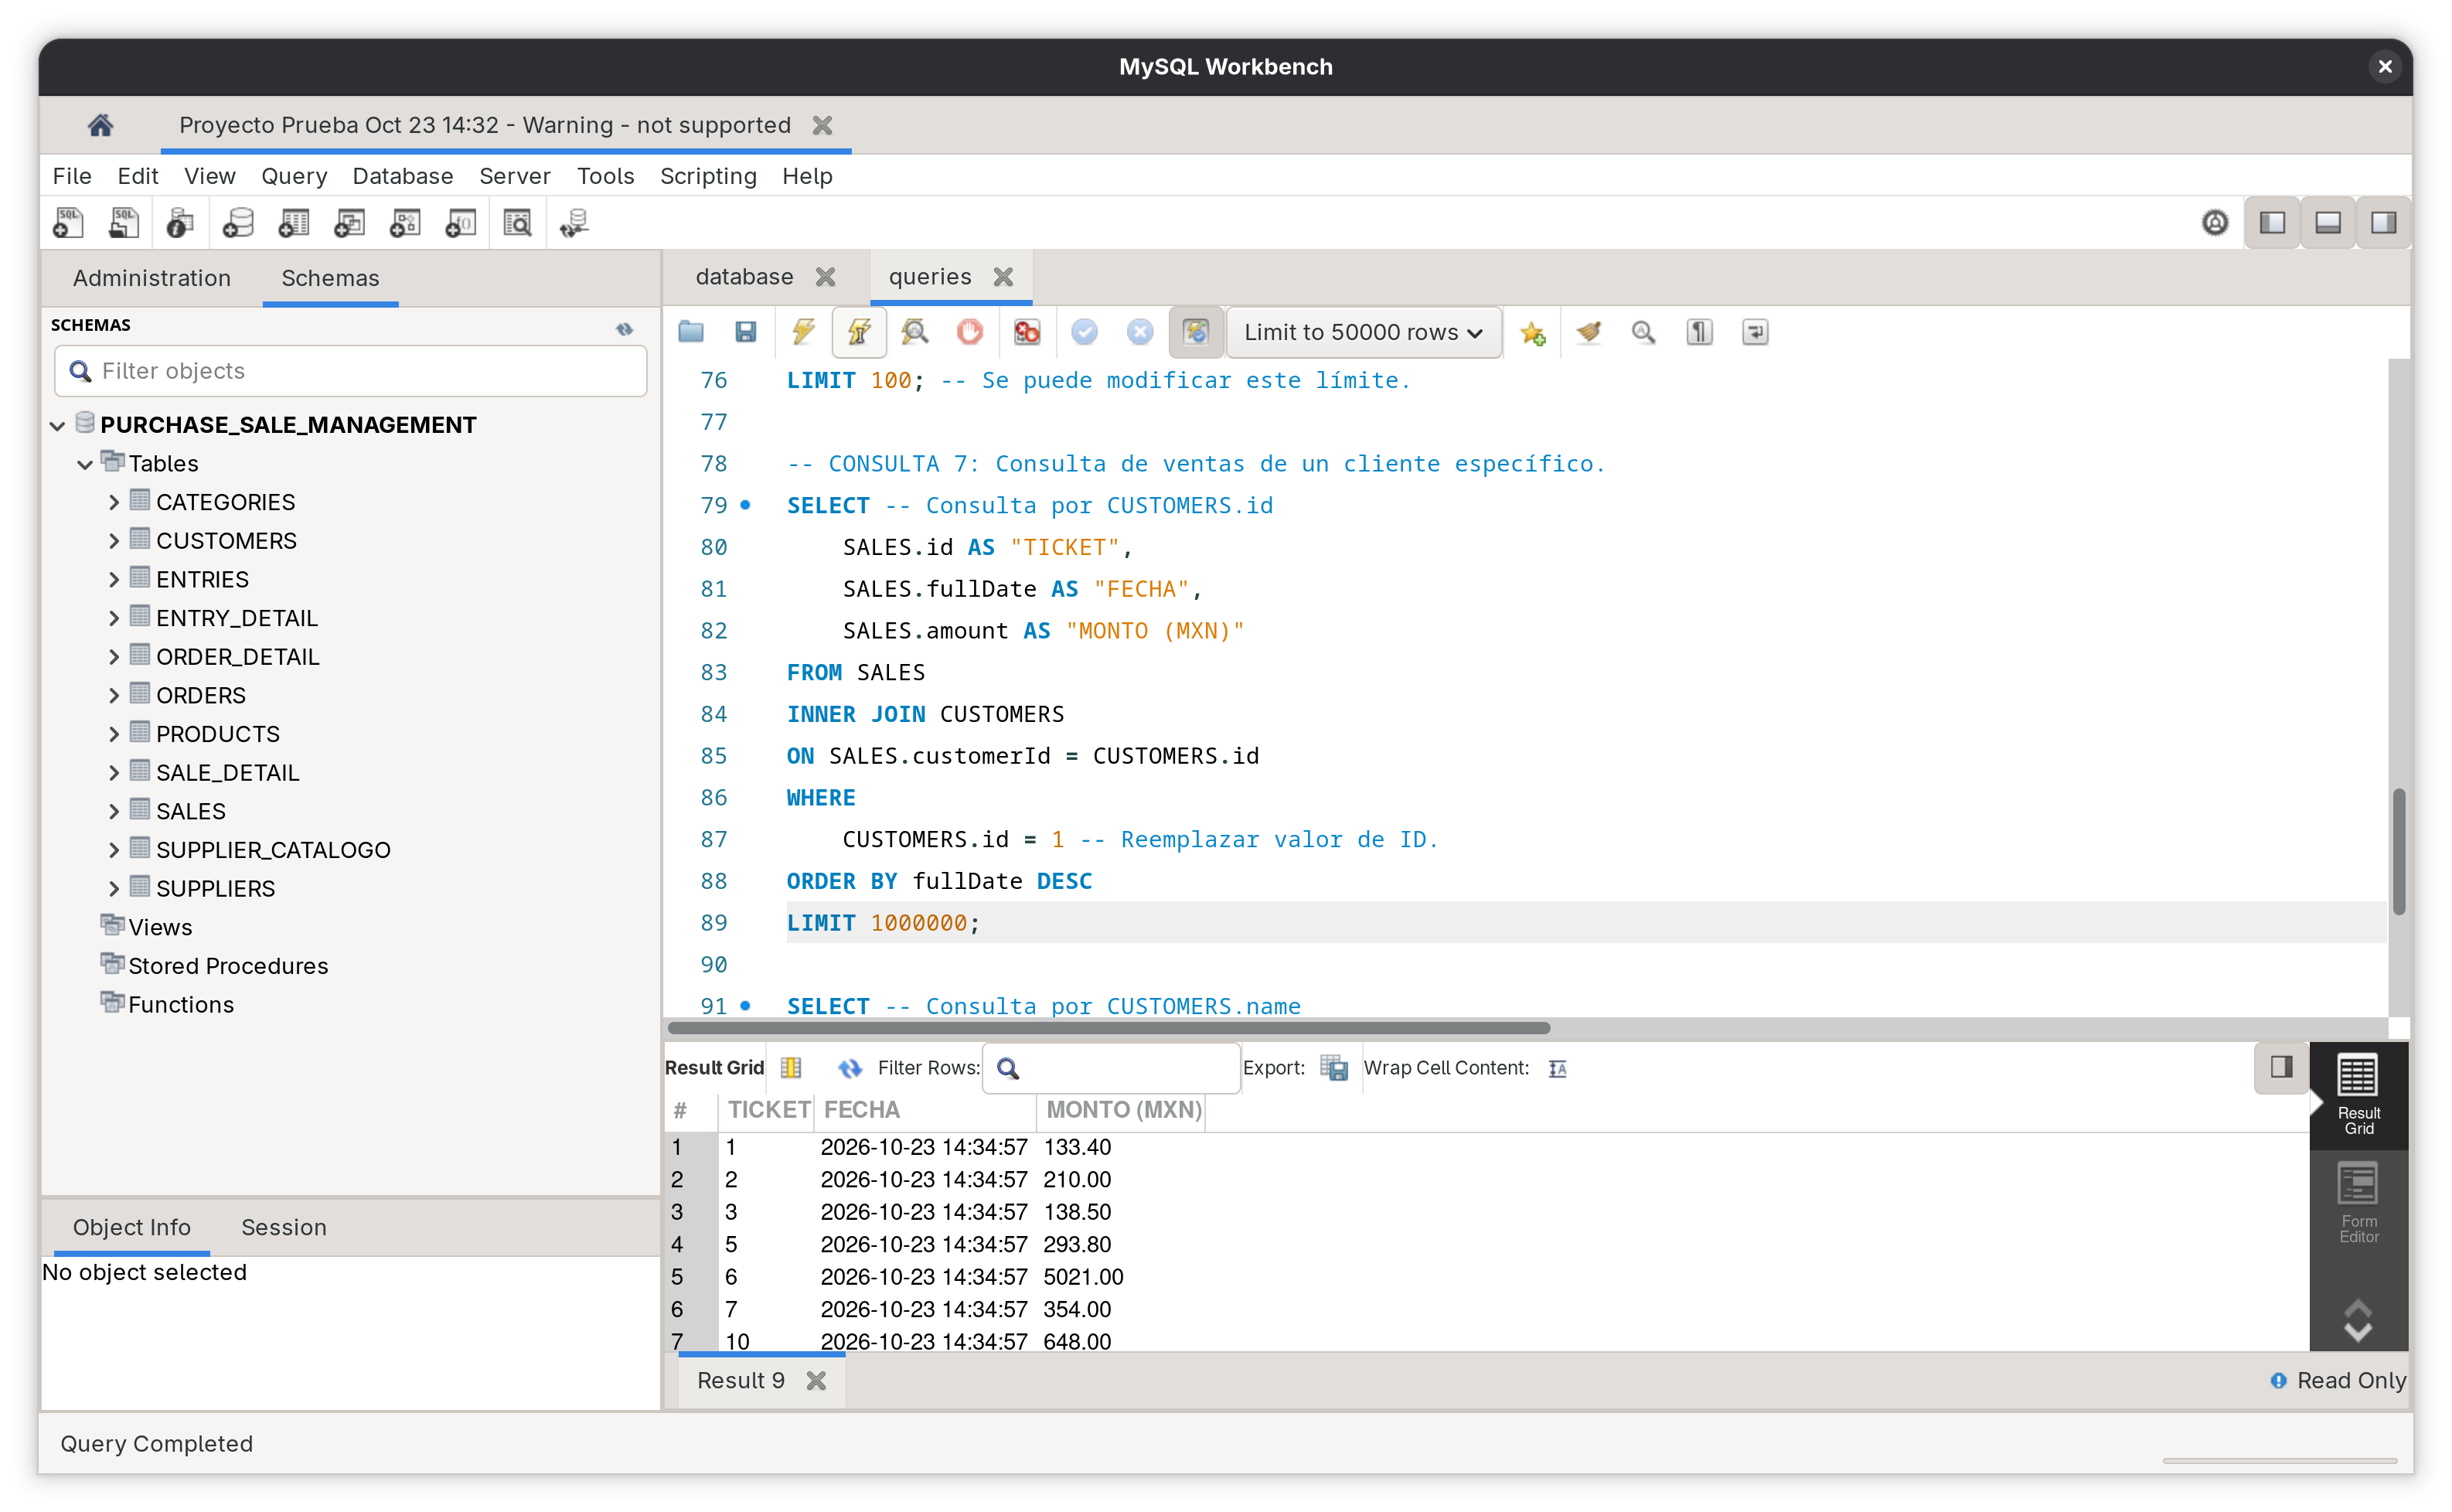
\includegraphics[
        width=0.9\linewidth
        ]{../img/evidencias/pruebas-consulta-7.png}
	\caption{\textit{Consulta 7}}
	\label{fig:consulta-7}
\end{figure}

\begin{figure}[!htb]
	\centering
	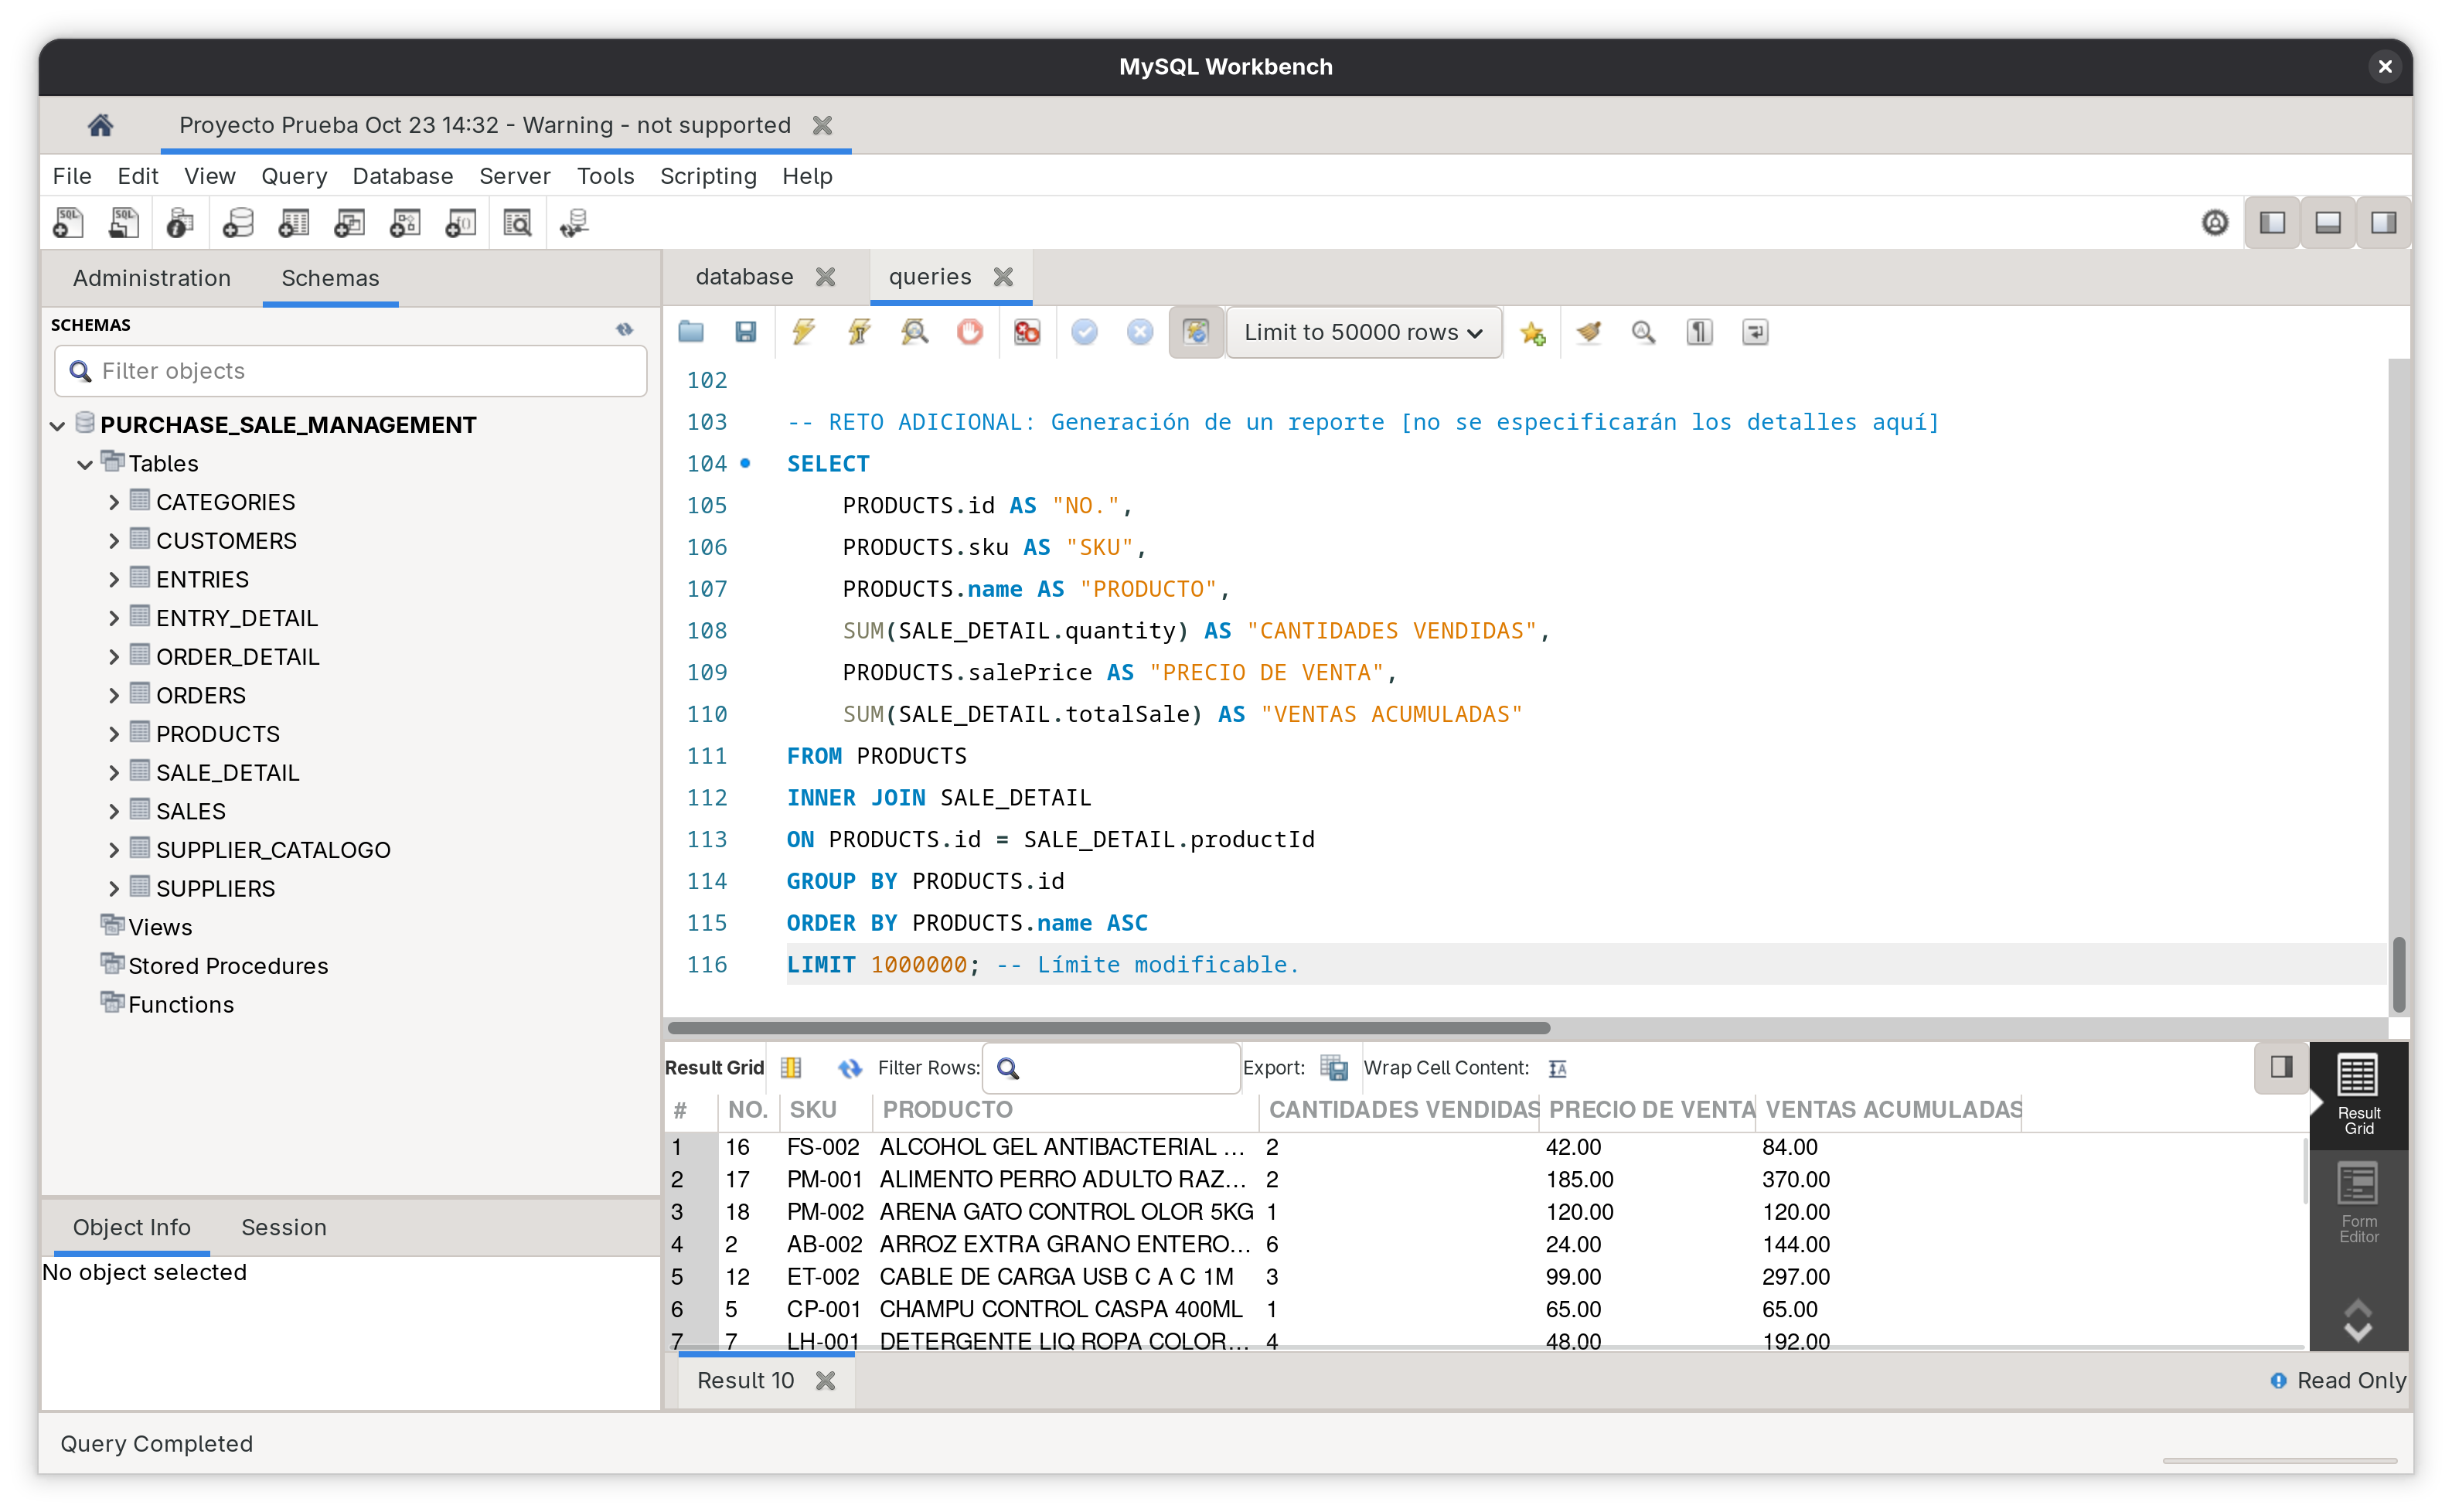
\includegraphics[
        width=0.9\linewidth
        ]{../img/evidencias/pruebas-reto-adicional.png}
	\caption{\textit{Reto adicional}}
	\label{fig:reto}
\end{figure}
\clearpage



\section*{\centering Justificación de diseño}
\addcontentsline{toc}{section}{Justificación de diseño}

\subsection*{\centering Problemática}
\addcontentsline{toc}{subsection}{Problemática}

Una tienda comercial necesita organizar la información de sus productos, proveedores, clientes y ventas. Actualmente, los registros se llevan de manera desordenada, lo que dificulta conocer las existencias, identificar los productos más vendidos y consultar los ingresos generados. Por ello, la tienda se ha propuesto utilizar una base de datos como la solución que le facilite controlar productos, proveedores, clientes, ventas y detalles de ventas, manteniendo la integridad y consistencia de la información generada en algunas de sus operaciones.
\newline

Por lo tanto, se diseñará y desarrollará una base de datos que permita a la tienda administrar la información comercial y facilitar la generación de reportes. 
\newline

Los empleados de la empresa deben poder ejecutar las siguientes operaciones:

\begin{itemize}
    \item \textbf{Listado} de todos los productos registrados.
    \item \textbf{Búsqueda} de productos por nombre o categoría.
    \item \textbf{Consulta} de las ventas realizadas.
    \item \textbf{Consulta} de los productos más vendidos.
    \item \textbf{Cálculo} del total de ventas por periodo.
    \item \textbf{Identificación} de productos con existencias bajas.
    \item \textbf{Consulta} de ventas de un cliente específico.
    \item Utilización de operaciones de inserción y consulta de datos.
    \item Generación de un reporte que muestre los productos vendidos, las cantidades, los precios y el importe total vendido por producto.
\end{itemize}

Los puntos o conceptos más importantes de la problemática de la tienda son: \texttt{base de datos}, \texttt{productos}, \texttt{proveedores}, \texttt{clientes}, \texttt{ventas}, \texttt{detalles de ventas}, \texttt{generación de reportes}, \texttt{operaciones en la base de datos}. Estos conceptos son el núcleo de lo que el usuario (la tienda comercial) solicita como fundamental y crítico en su petición. Por lo que se comprende que la tienda no requiere control relacionado con la gestión de empleados, nómina, contabilidad y otras áreas de operación y administración. Y también, se asumirá la operación de una sola tienda, la moneda será el \textbf{peso mexicano}, la zona horaria se considerará como base el horario de la ciudad de \textbf{Cancún}. En síntesis, la tienda requiere una base de datos para apoyar a su \textbf{proceso o ciclo de compra-venta}. 

\subsection*{\centering Del modelo relacional}
\addcontentsline{toc}{subsection}{Del modelo relacional}

Dada la información obtenida en el enunciado de la problemática, el sistema o proceso de la tienda comercial a modelar es el \textit{proceso o ciclo de compra-venta}. En tal modelo, los agentes y procesos principales son la \textbf{tienda}, el \textbf{producto}, el \textbf{inventario}, la \textbf{venta} , el \textbf{cliente} y el \textbf{proveedor}. Estos agentes y procesos se consideran parte de las entidades para un modelo relacional de bases de datos. Cabe añadir que las acciones de \textbf{vender} productos, \textbf{comprar} productos, \textbf{recepcionar} mercancía, \textbf{pedir} mercancía y \textbf{entregar} mercancía forman parte de los candidatos a relación.
\newline

De las entidades identificadas en la fase de desarrollo y diseño de la base de datos, se realiza un descarte de la entidad de \textbf{Existencias} por considerarse redundante con la existencia de la entidad de \textbf{Productos}. Esto se debe a que el primero únicamente guarda la relación de cantidades y su monto en precio de venta o costo y el segundo ya respalda las existencias de los productos y almacena los precios de costo y precio de venta.
\newline

Por decisión de simplificación, las entidades descritas en el modelo conceptual son \textit{fuertes}, ya que todas las anteriores se pueden identificar y existir por sí mismos, ya que son abstracciones de los agentes y procesos del proceso de compra-venta.
\newline

De igual forma, se identificaron y se crearon entidades asociativas como resultado a la solución de relaciones de cardinalidad \texttt{N:M}.

\subsection*{\centering De las restricciones de integridad}
\addcontentsline{toc}{subsection}{De las restricciones de integridad}

Se aplicó \texttt{NOT NULL} a los atributos que requieran una medida adicional para evitar introducir datos vacíos como las referencias de llaves foráneas u otros casos. En las llaves primarias no se aplicó \texttt{NOT NULL}, ya que estas por definición o restricción no pueden estar vacíos. Algunos atributos que pudieron ser candidatos a llave primaria así como datos de correos y números telefónicos se aplicó \texttt{UNIQUE} con la finalidad de evitar duplicaciones en campos de valores únicos o información de carácter unívoco. Por cuestiones de tiempo, no se preparó una política referencial como \texttt{ON DELETE} y \texttt{ON UPDATE} (\texttt{RESTRICT}, \texttt{CASCADE}, \texttt{SET NULL} ) y este es de lo detalles críticos que se han de trabajar en la siguiente ronda de desarrollo. Para finalizar este apartado, algunos atributos como los campos de precios y cantidades de productos (excepto en cuestión de existencias) se aplicaron reglas de dominio \texttt{CHECK} con la finalidad de que estos tengan valores decimales no negativos. Se permitió que las existencias de productos tenga \textbf{inventario negativo} debido a que es una práctica común desde el punto de vista administrativo, ya que facilita la rápida identificación de pérdidas en una tienda.

\subsection*{\centering De la normalización}
\addcontentsline{toc}{subsection}{De la normalización}

El diseño cumple la \textbf{primera forma normal (1FN)} debido a que cada tabla tiene una clave primaria y sus columnas representan atributos individuales, sin repetición de valores ni conjuntos dentro de cada fila. Los datos de las entidades (procesos y agentes del proceso de compra-venta) se separaron en tablas distintas, esto para evitar la redundancia de información en múltiples tablas. También, las relaciones \texttt{N:M} se resolvieron mediante entidades (tablas) asociativas que guardan los datos de cada relación. En otras palabras, es la primera manera y la más fundamental de evitar duplicación de información aun cuando se trate de bases de datos con pocas entidades o escasa complejidad.
\newline

La \textbf{segunda forma normal (2FN)} implica que las claves primarias, en este diseño, se dividan en simples o compuestas; las simples para las entidades fuertes y las compuestas para las entidades asociativas. Estas claves permiten la identificación de cada uno de los registros. En las entidades asociativas, la combinación de claves permite identificar la relación de las operaciones y las entidades sin que haya que depender de información redundante. Además, las claves foráneas permiten referenciar las tablas de origen, en lugar de estar duplicando en cada registro la información que contiene la tabla de origen.
\newline

La \textbf{tercera forma normal (3FN)} implica el mantener los datos descriptivos en sus tablas correspondientes y referenciarlos mediante claves, evitando que atributos no clave dependan de otros atributos no clave. Es decir, que datos que se puedan calcular, recalcular y obtener mediante ciertas operaciones como las aritméticas cuyos operandos sean los mismos atributos no claves no deberían almacenarse en las tablas, basta con conservar los operandos sin registrar el resultado. Esto no ocurre en este diseño de base de datos, o al menos en la mayor parte de los atributos. Esto se ha dejado así (como los cálculos de costos, detalles de ventas, cálculo de stock) para facilitar el registro y consulta de datos para la generación de reportes que requiera la tienda comercial.
\newline

Por lo tanto, no se cumple la \textbf{3FN} de forma estricta, mientras que \textbf{1FN} y \textbf{2FN} sí. Dado que no se normalizó, de manera deliberada, bajo la tercera forma normal por decisiones de diseño, el esquema relacional está normalizado hasta donde corresponde.

\subsection*{\centering De las operaciones de inserción}
\addcontentsline{toc}{subsection}{De las operaciones de inserción}

La primera inserción de datos habilita la base de datos para su primer y posteriores usos. Para operar la tienda primero se deben definir las categorías de productos (\textbf{categoría general} es la clasificación obligatoria), dar de alta los productos y después a los proveedores. Una vez hecho esto, ya se genera el catálogo de los proveedores y la lista de los clientes (donde el cliente primero y obligatorio es \textbf{público general}).
\newline

Una vez hecho lo anterior, se generan pedidos a los proveedores, se da de alta las entradas de mercancía y la modificación de las existencias de los productos. En paralelo, se generan los detalles de los primeros pedidos, luego el de la recepción. Con ello queda listo el stock para vender.
\newline

Luego se realiza una venta, se emite el detalle de una venta. A partir de aquí se puede realizar las operaciones del proceso de compra-venta: pedidos (y sus detalles), recepciones (y sus detalles), alta de proveedores y productos, alta de clientes, ventas (y detalles). Las correcciones y bajas de pedidos, recepciones, productos, clientes y ventas aún no se pueden realizar de manera fiable.

\newpage
\listoftables
\listoffigures

\end{document}